% CSE 150A/250A Final Project Report
% Due: Mon Nov 23, 11:59 PM PT (Gradescope). Optional resubmission: Fri Dec 11, 2:59 PM PT.
% Limit: 7 content pages (Sections 1--6). References and appendices don't count.
%
% Build:  cd paper/report && latexmk -pdf main.tex
\documentclass[11pt]{article}
% Shared preamble for the proposal and the report.
% Loaded from each main.tex with % Shared preamble for the proposal and the report.
% Loaded from each main.tex with % Shared preamble for the proposal and the report.
% Loaded from each main.tex with \input{../common/preamble}.

% --- Page style ---------------------------------------------------------------
% The course recommends the NeurIPS style. Download the style file from the
% NeurIPS / Overleaf template and drop neurips_20XX.sty into paper/common/.
% If it's missing, we fall back to a plain 1-inch-margin article so everything
% still compiles.
\makeatletter
\IfFileExists{../common/neurips_2026.sty}{%
  \usepackage[final]{../common/neurips_2026}\def\cse@neurips{}}{%
\IfFileExists{../common/neurips_2025.sty}{%
  \usepackage[final]{../common/neurips_2025}\def\cse@neurips{}}{%
  \usepackage[margin=1in]{geometry}%
  \usepackage{natbib}%
}}
\makeatother

% --- Packages -----------------------------------------------------------------
\usepackage[utf8]{inputenc}
\usepackage[T1]{fontenc}
\usepackage{amsmath, amssymb, amsfonts}
\usepackage{bm}                 % bold math: \bm{x}
\usepackage{graphicx}
\usepackage{booktabs}           % nice tables: \toprule \midrule \bottomrule
\usepackage{subcaption}
\usepackage{placeins}        % \FloatBarrier: keep appendix figures in their section
\usepackage{xcolor}
% Scalable fonts let microtype do full typesetting tweaks; minimal TeX installs
% without lmodern still compile, just without font expansion.
\IfFileExists{lmodern.sty}{\usepackage{lmodern}\usepackage{microtype}}{\usepackage[expansion=false]{microtype}}
\usepackage{url}
\usepackage[hidelinks]{hyperref}
\usepackage{cleveref}           % \cref{fig:x} -> "Figure 1"
\usepackage{enumitem}           % list options: [label=..., leftmargin=*]

% Figures generated by code live in the repo's figures/ folder.
\graphicspath{{../../../figures/}{../figures/}}

% --- Project macros -----------------------------------------------------------
% Draft notes. Search for \todo before submitting. Set to {} to hide all of them.
\newcommand{\todo}[1]{\textcolor{red}{[TODO: #1]}}

% Notation (keep consistent across sections)
\newcommand{\given}{\mid}
\newcommand{\Prob}{P}
\DeclareMathOperator*{\argmax}{arg\,max}

% Shared layout for the per-phase Methodology subsections.
\input{../common/phase-macros}
.

% --- Page style ---------------------------------------------------------------
% The course recommends the NeurIPS style. Download the style file from the
% NeurIPS / Overleaf template and drop neurips_20XX.sty into paper/common/.
% If it's missing, we fall back to a plain 1-inch-margin article so everything
% still compiles.
\makeatletter
\IfFileExists{../common/neurips_2026.sty}{%
  \usepackage[final]{../common/neurips_2026}\def\cse@neurips{}}{%
\IfFileExists{../common/neurips_2025.sty}{%
  \usepackage[final]{../common/neurips_2025}\def\cse@neurips{}}{%
  \usepackage[margin=1in]{geometry}%
  \usepackage{natbib}%
}}
\makeatother

% --- Packages -----------------------------------------------------------------
\usepackage[utf8]{inputenc}
\usepackage[T1]{fontenc}
\usepackage{amsmath, amssymb, amsfonts}
\usepackage{bm}                 % bold math: \bm{x}
\usepackage{graphicx}
\usepackage{booktabs}           % nice tables: \toprule \midrule \bottomrule
\usepackage{subcaption}
\usepackage{placeins}        % \FloatBarrier: keep appendix figures in their section
\usepackage{xcolor}
% Scalable fonts let microtype do full typesetting tweaks; minimal TeX installs
% without lmodern still compile, just without font expansion.
\IfFileExists{lmodern.sty}{\usepackage{lmodern}\usepackage{microtype}}{\usepackage[expansion=false]{microtype}}
\usepackage{url}
\usepackage[hidelinks]{hyperref}
\usepackage{cleveref}           % \cref{fig:x} -> "Figure 1"
\usepackage{enumitem}           % list options: [label=..., leftmargin=*]

% Figures generated by code live in the repo's figures/ folder.
\graphicspath{{../../../figures/}{../figures/}}

% --- Project macros -----------------------------------------------------------
% Draft notes. Search for \todo before submitting. Set to {} to hide all of them.
\newcommand{\todo}[1]{\textcolor{red}{[TODO: #1]}}

% Notation (keep consistent across sections)
\newcommand{\given}{\mid}
\newcommand{\Prob}{P}
\DeclareMathOperator*{\argmax}{arg\,max}

% Shared layout for the per-phase Methodology subsections.
% phase-macros.tex — shared macros for per-phase Methodology sections.
% Loaded by common/preamble.tex (after graphicx), so every main.tex gets them.

% Phase heading with an automatic label: \phasesection{1}{Single-gas BN (MLE)}
% Creates \subsection{Phase 1: ...} labeled sec:phase-1.
\newcommand{\phasesection}[2]{%
  \subsection{Phase #1: #2}\label{sec:phase-#1}}

% Bold run-in heading for each part of a phase: \phasepart{Goal}
\newcommand{\phasepart}[1]{\paragraph{#1.}}

% Phase figure: \phasefigure{1}{phase-1.jpg}{Caption text.}
% Optional width (default 0.6\linewidth), e.g. for the wide HMM figure:
%   \phasefigure[\linewidth]{4}{phase-4.jpg}{Caption text.}
% Labeled fig:phase-<n>; reference with Figure~\ref{fig:phase-1}.
\newcommand{\phasefigure}[4][0.6\linewidth]{%
  \begin{figure}[t]
    \centering
    \includegraphics[width=#1]{#3}
    \caption{#4}
    \label{fig:phase-#2}
  \end{figure}}

.

% --- Page style ---------------------------------------------------------------
% The course recommends the NeurIPS style. Download the style file from the
% NeurIPS / Overleaf template and drop neurips_20XX.sty into paper/common/.
% If it's missing, we fall back to a plain 1-inch-margin article so everything
% still compiles.
\makeatletter
\IfFileExists{../common/neurips_2026.sty}{%
  \usepackage[final]{../common/neurips_2026}\def\cse@neurips{}}{%
\IfFileExists{../common/neurips_2025.sty}{%
  \usepackage[final]{../common/neurips_2025}\def\cse@neurips{}}{%
  \usepackage[margin=1in]{geometry}%
  \usepackage{natbib}%
}}
\makeatother

% --- Packages -----------------------------------------------------------------
\usepackage[utf8]{inputenc}
\usepackage[T1]{fontenc}
\usepackage{amsmath, amssymb, amsfonts}
\usepackage{bm}                 % bold math: \bm{x}
\usepackage{graphicx}
\usepackage{booktabs}           % nice tables: \toprule \midrule \bottomrule
\usepackage{subcaption}
\usepackage{placeins}        % \FloatBarrier: keep appendix figures in their section
\usepackage{xcolor}
% Scalable fonts let microtype do full typesetting tweaks; minimal TeX installs
% without lmodern still compile, just without font expansion.
\IfFileExists{lmodern.sty}{\usepackage{lmodern}\usepackage{microtype}}{\usepackage[expansion=false]{microtype}}
\usepackage{url}
\usepackage[hidelinks]{hyperref}
\usepackage{cleveref}           % \cref{fig:x} -> "Figure 1"
\usepackage{enumitem}           % list options: [label=..., leftmargin=*]

% Figures generated by code live in the repo's figures/ folder.
\graphicspath{{../../../figures/}{../figures/}}

% --- Project macros -----------------------------------------------------------
% Draft notes. Search for \todo before submitting. Set to {} to hide all of them.
\newcommand{\todo}[1]{\textcolor{red}{[TODO: #1]}}

% Notation (keep consistent across sections)
\newcommand{\given}{\mid}
\newcommand{\Prob}{P}
\DeclareMathOperator*{\argmax}{arg\,max}

% Shared layout for the per-phase Methodology subsections.
% phase-macros.tex — shared macros for per-phase Methodology sections.
% Loaded by common/preamble.tex (after graphicx), so every main.tex gets them.

% Phase heading with an automatic label: \phasesection{1}{Single-gas BN (MLE)}
% Creates \subsection{Phase 1: ...} labeled sec:phase-1.
\newcommand{\phasesection}[2]{%
  \subsection{Phase #1: #2}\label{sec:phase-#1}}

% Bold run-in heading for each part of a phase: \phasepart{Goal}
\newcommand{\phasepart}[1]{\paragraph{#1.}}

% Phase figure: \phasefigure{1}{phase-1.jpg}{Caption text.}
% Optional width (default 0.6\linewidth), e.g. for the wide HMM figure:
%   \phasefigure[\linewidth]{4}{phase-4.jpg}{Caption text.}
% Labeled fig:phase-<n>; reference with Figure~\ref{fig:phase-1}.
\newcommand{\phasefigure}[4][0.6\linewidth]{%
  \begin{figure}[t]
    \centering
    \includegraphics[width=#1]{#3}
    \caption{#4}
    \label{fig:phase-#2}
  \end{figure}}



\title{Estimating True Air Pollution from Noisy Low-Cost Sensors}
% Shared author block. Fill in missing names/emails.
\author{%
  Kiernan Beresford \\ UC San Diego \\ \texttt{kberesfo@ucsd.edu} \and
  Agnes \todo{last name} \\ UC San Diego \\ \texttt{\todo{email}} \and
  Zachary Brown \\ UC San Diego \\ \texttt{z5brown@ucsd.edu} \and
  Muska Mesdaq \\ UC San Diego \\ \texttt{\todo{email}} \and
  Joyce Yang \\ UC San Diego \\ \texttt{\todo{email}}
}

\date{}

\begin{document}
\maketitle

\begin{abstract}
  Low-cost sensors are cheap enough to deploy widely, but their
  readings drift with weather and respond to more than one gas, so they do not
  directly measure true pollution. Using one year of hourly data from a
  road-level multisensor device with a co-located reference analyzer (UCI Air
  Quality), we estimate the true levels of CO, NO$_x$ and NO$_2$ from only what
  a deployed device observes: hour of day, weather and its own sensors. Our
  model is a discrete Bayesian network with cross-sensitivity edges and a
  latent emission regime, learned with EM from partially observed references.
  It reduces concentration error relative to an hour-of-day baseline by
  37\%, 32\% and 18\% for CO, NO$_x$ and NO$_2$. The regime
  explains most of the co-movement between gases and improves the joint fit, 
  capturing shared structure that per-gas metrics do not show. 
\end{abstract}

\section{Problem Description}
\label{sec:problem}
% ~0.5 page. Models: hour-only baseline, Phase 1, Phase 3b (final).

Reference stations measure urban air pollution accurately but are expensive,
so cities have few of them. Low-cost metal-oxide sensors could fill the gaps,
but they are noisy, drift, and respond to weather and to gases other than their
target, so they must be calibrated in the field against a reference
\citep{devito2008calibration}. We treat calibration as probabilistic
inference: the true concentration is latent, and the sensors are noisy,
indirect observations of it. A co-located reference analyzer provides ground
truth for training, but its CO, NO$_x$ and NO$_2$ records are missing on
17--18\% of hours (\cref{sec:data}). A Bayesian network suits this setting:
the dependencies among gases, sensors and weather form a directed graph, EM
\citep{dempster1977em} learns from the partially observed references, and
exact inference returns a posterior over each pollution level.

\paragraph{Research questions.} Using only what a deployed device observes
(hour, weather and its own sensors), never a reference reading:
\textbf{Q1 (estimation):} can a discrete BN learned with EM estimate pollution
better than the hour of day alone, and how close does it come to the limit set
by discretization? \textbf{Q2 (shared structure):} the gases come from the
same traffic and rise and fall together; does a latent emission regime capture
that co-movement, and does it improve the estimates?

\paragraph{Approach and findings.} We compare an hour-of-day baseline, a
single-gas network for CO (Phase~1) and our final model (Phase~3b), which
estimates CO, NO$_x$ and NO$_2$ jointly through a latent regime, with sensor
edges chosen by a cross-sensitivity study (\cref{app:cross}). On held-out test
weeks the final model cuts the baseline's error by 37\% for CO, 32\% for
NO$_x$ and 18\% for NO$_2$, closing 87\% and 71\% of the gap to the
discretization floor for CO and NO$_x$ but only 39\% for NO$_2$. The regime
explains most of the gases' co-movement but mainly improves NO$_2$.
\section{Data Sourcing and Processing}
\label{sec:data}
% ~1 page. Start from the proposal's Dataset section.
%
% - Source: UCI Air Quality \citep{vito2008airquality, devito2008calibration};
%   9,357 hours, Mar 2004--Feb 2005, one roadside device.
% - Variables table: kept / dropped / role (input, partially observed, observed).
% - Missing data: -200 -> NaN; fraction missing per column (CO 18%,
%   NOx/NO2 17.5%, NMHC 90%); reference gaps handled by EM, hours with missing
%   weather dropped (366) because inputs have no CPT.
% - Feature selection (cite App. cross-sensitivity study):
%     NMHC dropped (90% missing); C6H6 dropped (deterministic function of S2);
%     S2 dropped (no remaining gas parent); W = T + RH.
% - Discretization: quantile bins fit on train; K = 3 default; bin count
%   compared in Sec. 4 (3 vs 7).
% - CHANGED from proposal: split is blocked by week (weeks shuffled into
%   train/val/test), not one time cut; val for every choice, test once.
%   Say why: neighbouring hours are near-duplicates.
% - Limitations: one device, one site, one year; drift not modeled.

\section{Modeling and Inference}
\label{sec:modeling}
% ~1.75 pages. One figure (network), one equation per subsection.
\subsection{Bayesian Network}
\label{sec:bn}

\paragraph{Variables.} Each hour $t$ is described by the hour of day
$H \in \{0,\dots,23\}$, a weekday indicator $D \in \{0,1\}$, the weather
$W = (T, \mathit{RH})$, the reference gases
$G = (G_{\mathrm{CO}}, G_{\mathrm{NO_x}}, G_{\mathrm{NO_2}})$ and the sensors
$S = (S_1, S_3, S_4, S_5)$. Every continuous variable is discretized into $K$
quantile bins fit on the training split (Sec.~\ref{sec:data}); $K = 3$ unless
stated. The gases are partially observed in training and always hidden at
prediction time; $H$, $D$ and $W$ are always observed.

\paragraph{Structure.} The network (\cref{fig:network}) factorizes as
\begin{equation}
  P(G, S \mid H, W) = \prod_{j} P(G_j \mid H)
  \prod_{i} P\bigl(S_i \mid \mathrm{Pa}_G(S_i), T, \mathit{RH}\bigr),
  \label{eq:factorization}
\end{equation}
where $\mathrm{Pa}_G(S_i)$ are the gases sensor $i$ responds to. The inputs have
no CPTs; we only condition on them. Each edge type has a physical reason:
hour $\to$ gas captures the daily traffic cycle; gas $\to$ sensor links each
sensor to its nominal target \citep{devito2008calibration} ($S_1$: CO, $S_3$:
NO$_x$, $S_4$: NO$_2$); and weather $\to$ sensor reflects the metal-oxide
sensors' dependence on temperature and humidity. $S_5$'s nominal target, O$_3$,
has no reference, so its gas parents come from data alone. The
cross-sensitivity edges (CO, NO$_x$ $\to S_4$ and $S_5$) were added by forward
selection only if they raised held-out log-likelihood and kept a partial
correlation with the sensor in all three split seeds (\cref{app:cross}). NMHC
(90\% missing), C$_6$H$_6$ (an almost exact function of $S_2$) and $S_2$
itself are excluded. Earlier phases are subgraphs of this one
(\cref{app:networks}).

\paragraph{Assumptions.} \Cref{eq:factorization} assumes that the gases are
independent given the hour, that each sensor is independent of the others
given its parents, and that hours are independent with one set of CPTs for the
whole year. The first is the strongest, since all three gases come from
traffic; \cref{sec:latent} relaxes it. The second means a signal shared by
several sensors is counted once per sensor, making the posterior
overconfident (\cref{sec:results}). The third ignores autocorrelation and
sensor drift.

\paragraph{Parameters.} A node with $K_X$ states and parent configurations
$\prod K_U$ has $(K_X - 1)\prod K_U$ free parameters. At $K = 3$ the network has
900, and $S_4$, with five parents, accounts for 486 of them.

\begin{figure}[t]
  \centering
  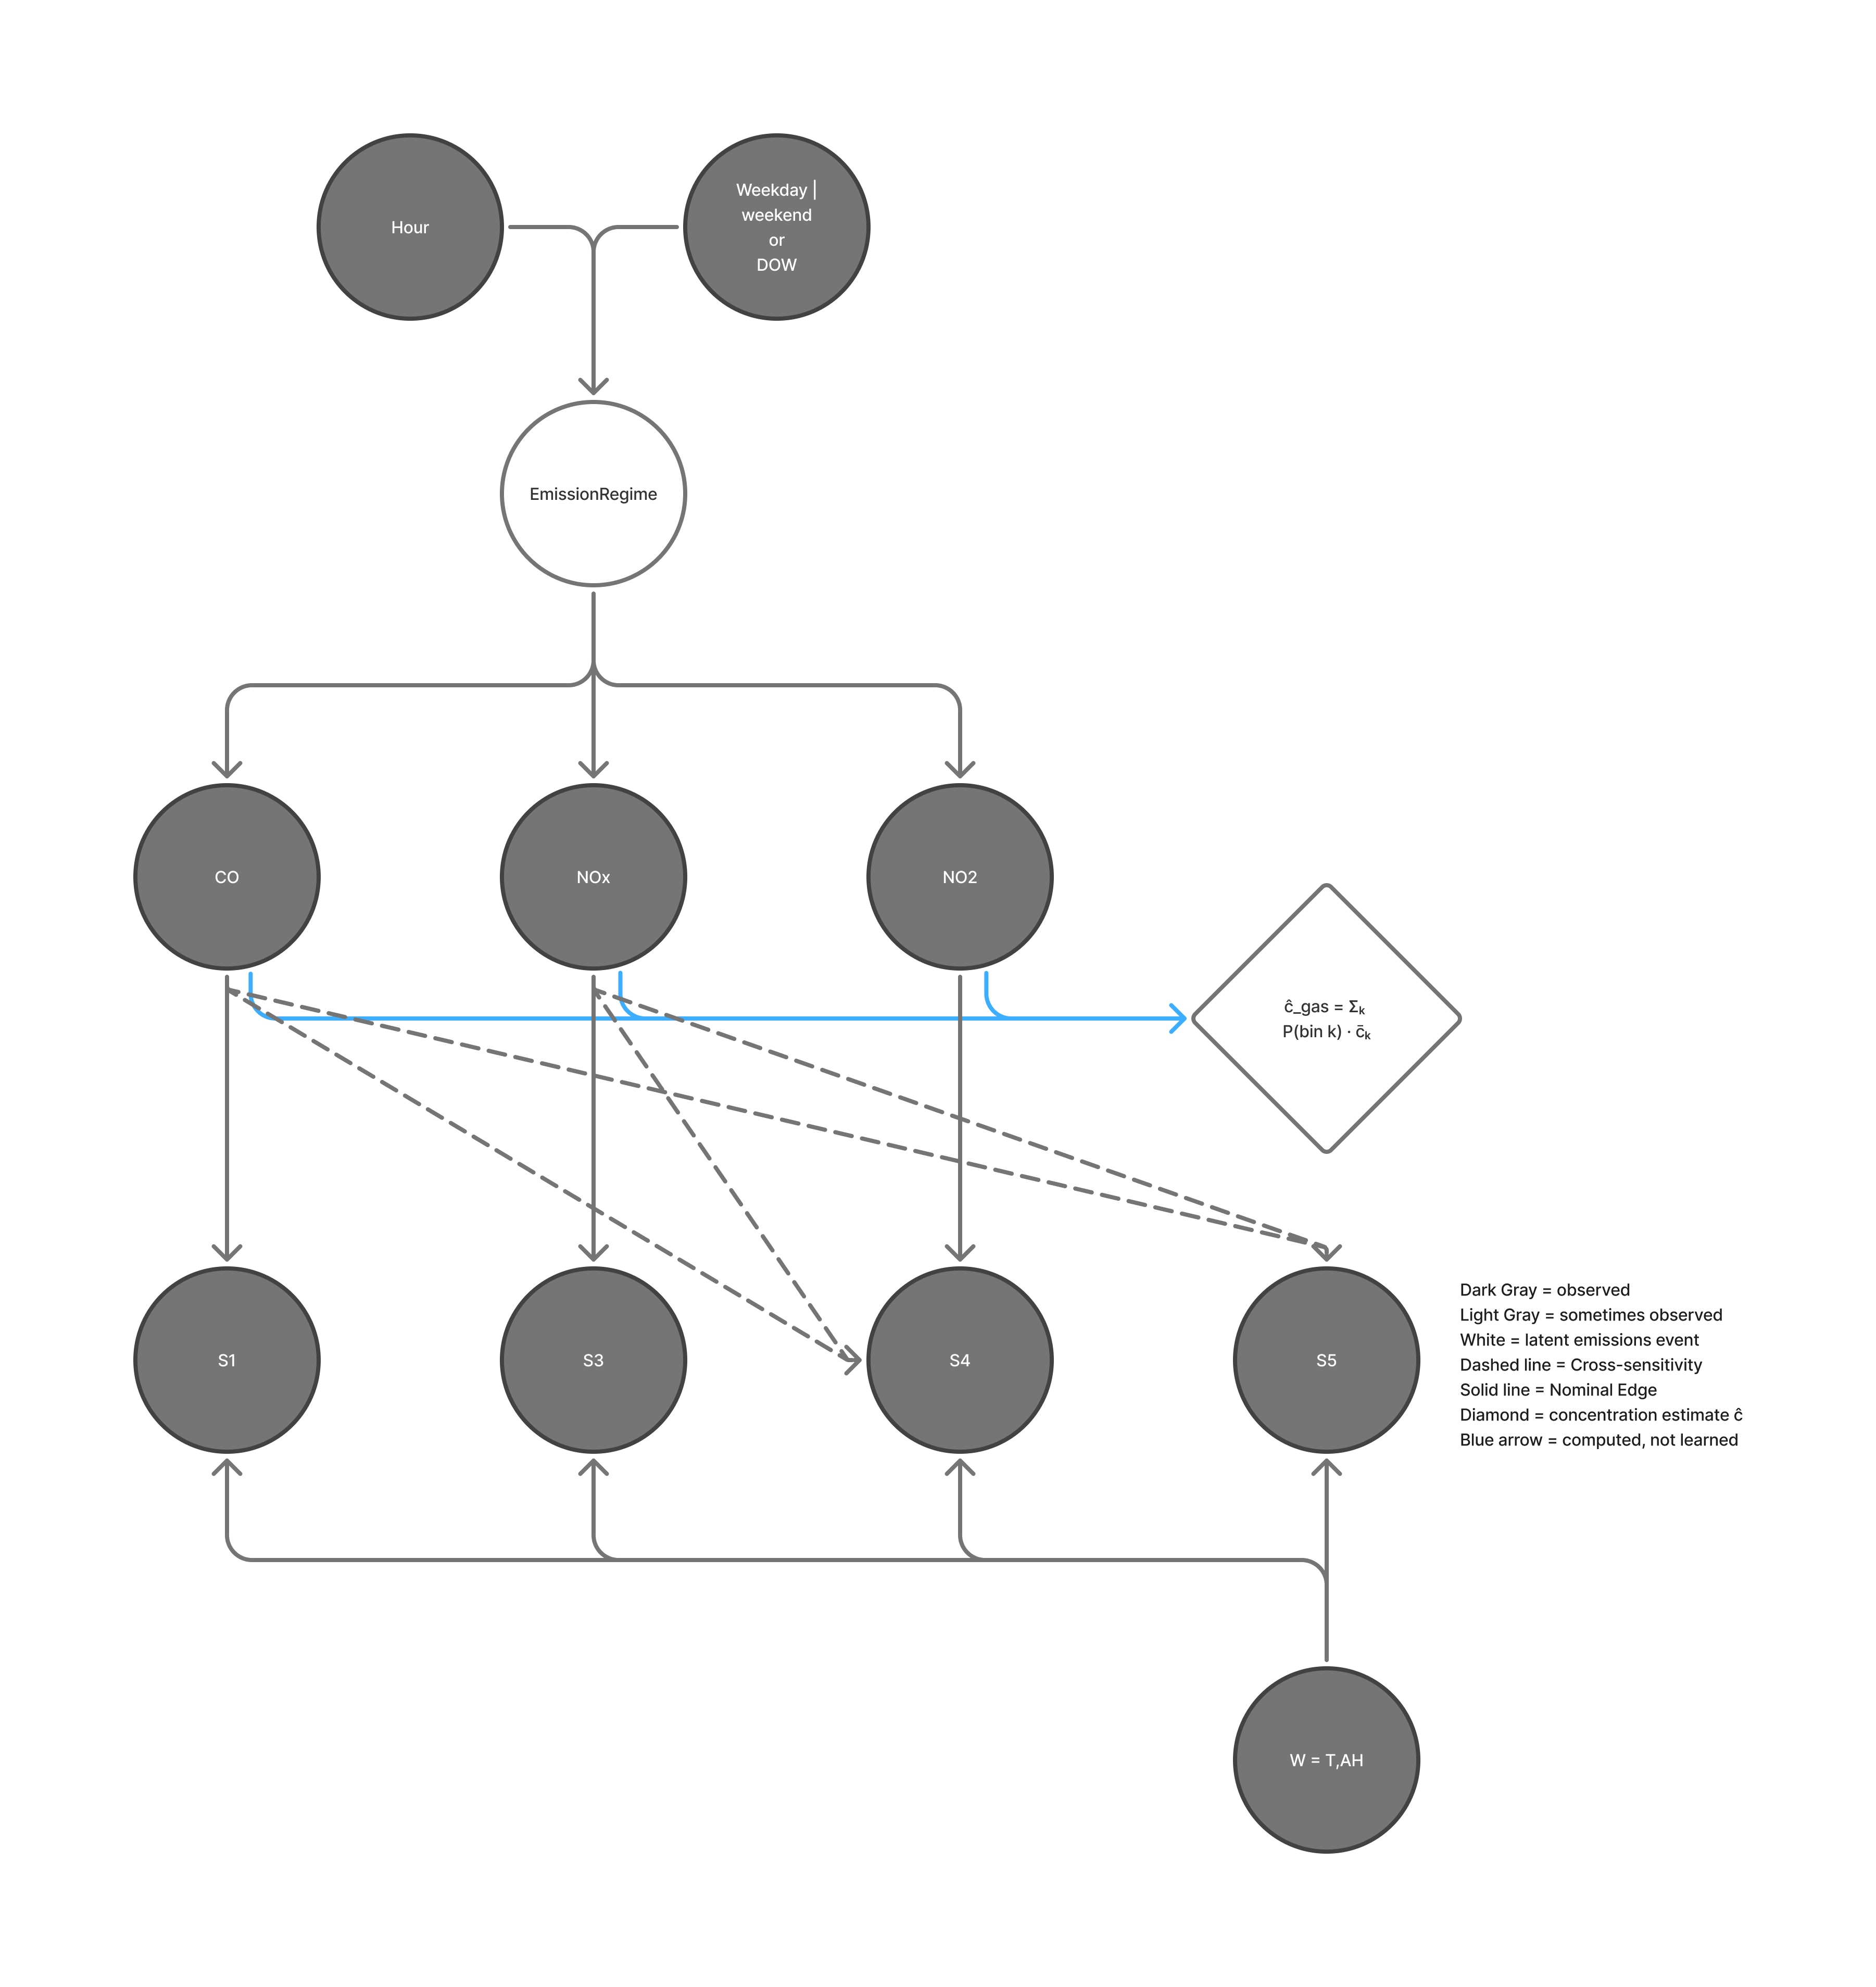
\includegraphics[width=0.6\linewidth]{phase-3b}
  \caption{Final network. Solid edges: nominal sensor targets; dashed: 
  cross-sensitivities selected from data; $R$ is the latent emission regime
  (\cref{sec:latent}). The diamond is air quality, derived from the estimated
  concentrations rather than modeled.}
  \label{fig:network}
\end{figure}


\subsection{Latent Emission Regime}
% - R <- hour, weekday; gases <- R. Unobserved on every row.
% - Purpose: make gases conditionally independent (check: within-R corr ~ 0).
% - K_R chosen by val log-lik + restart stability.
\todo{muska}

\subsection{Learning with Missing Data (EM)}
\label{sec:em}

\paragraph{What is missing.} Hour is always recorded. The sensors and weather
go missing together, during whole-device outages on 3.9\% of hours; we drop
those 366 hours (8,991 remain), which leaves the sensors fully observed and the
inputs complete, since inputs have no CPT and cannot be inferred. The reference gases are
missing far more often: CO on 18.0\% of hours and NO$_x$ and NO$_2$ on 17.5\%.
These gaps are concentrated at night, peaking at 54\% of CO readings at 4\,AM
and 93\% of NO$_2$ readings at 3\,AM, consistent with a scheduled analyzer
calibration. Because the missingness depends on the hour, which the model
conditions on, rather than on the concentration itself, we treat the gaps as
missing at random \citep{dempster1977em}. The latent regime $R$ has no column
and is missing on every hour.

\paragraph{EM.} Rather than imputing missing values, EM averages over them. In
the E-step, each training hour contributes expected counts
$\hat N(x,u) = \sum_t P(X{=}x, U{=}u \mid e_t; \theta)$ to every family
$(X, U)$: an indicator where the family is observed, and the current posterior
over the missing values where it is not. The M-step re-estimates each CPT row
from these counts with Laplace smoothing ($\alpha = 1$):
\begin{equation}
  \theta_{x \mid u} = \frac{\hat N(x,u) + \alpha}{\sum_{x'} \hat N(x',u) + K_X \alpha}.
\end{equation}
This is MAP estimation under a Dirichlet prior, so EM is guaranteed never to
decrease the objective $\mathcal{L}$, the log-likelihood plus log-prior.

\paragraph{Initialization and convergence.} CPTs of nodes with data start from
smoothed counts on the hours where their family is fully observed; the latent
regime $R$ starts from random tables drawn with a fixed seed. EM stops when an
iteration improves $\mathcal{L}$ by less than a relative tolerance,
$\mathcal{L}^{(s)} - \mathcal{L}^{(s-1)} < \epsilon\,\lvert \mathcal{L}^{(s-1)} \rvert$
with $\epsilon = 10^{-4}$, or after 100 iterations. We record $\mathcal{L}$ at
every iteration and check that it never decreases beyond round-off; a decrease
would indicate an implementation error. Phase~1 converges in 3 iterations
because CO is observed on 82\% of hours.

\paragraph{Stability of the latent regime.} With $R$ fully hidden, the
objective has several local optima, and the same regimes can come out in a
different order on each run (label switching). We run several restarts, match
states across runs by their gas profiles (Hungarian matching), and accept a
number of regimes $K_R$ only if the matched states agree across restarts. That
way the regimes mean the same thing every time we fit and can be interpreted
(\cref{sec:results}).

\subsection{Inference}
% - Query P(G_j | hour, weekday, W, sensors); reference never evidence.
% - Exact by enumeration over hidden joint (K_R * K^3 states); cost linear in N.
% - Concentration estimate = sum_k P(bin k | e) c_bar_k; resolution floor.
\todo{yang \& muska}
\section{Results and Discussion}
\label{sec:results}

% ~2.5 pages (gets the space freed by dropping the HMM).
% Organize by research question; every number comes from
% notebooks/<phase>/eval.ipynb -> results/<phase>/ and its [Exp] issue.
% Report val for every comparison; test once, in the main table only.

\subsection{Experimental Setup}
\label{sec:setup}
Splits are blocked by week into train, validation and test, repeated for seeds 0, 1 and 2.
Every choice (bin count, edges, $K$) is made on validation; test is scored once, after
refitting on train plus validation.

We score the concentration estimate $\hat{c}=\sum_k P(\mathrm{bin}_k\mid e)\,\bar{c}_k$
by its mean absolute error (MAE), in each gas's units (CO in mg/m$^3$, NO$_x$ in ppb,
NO$_2$ in $\mu$g/m$^3$). The \emph{resolution floor} is the MAE of an oracle that knows the true bin
and outputs its mean. We report
\[
\text{skill}=1-\frac{\mathrm{MAE}_{\text{model}}}{\mathrm{MAE}_{\text{baseline}}},\qquad
\text{gap closed}=\frac{\mathrm{MAE}_{\text{baseline}}-\mathrm{MAE}_{\text{model}}}
{\mathrm{MAE}_{\text{baseline}}-\mathrm{MAE}_{\text{floor}}},
\]
which are unitless and so comparable across gases. The baseline is hour of day only, with the same
evidence interface. The mean log-likelihood of the true bin is a secondary metric and is only
comparable at the same bin count. Numbers are mean $\pm$ std over the three seeds.

\subsection{Q1: Estimation}
\label{sec:q1}
% TODO(Muska's run): fill the -- cells from results/final/test_grid.csv; set headline bin count.
\begin{table}[htbp]
\centering
\caption{Test concentration error (mean $\pm$ std over seeds). Phase 1 models CO only.}
\label{tab:main}
\begin{tabular}{llcccc}
\toprule
Gas & Model & MAE & Floor & Skill & Gap closed \\
\midrule
CO & Hour baseline & -- & -- & -- & -- \\
   & Phase 1       & -- & -- & -- & -- \\
   & Phase 3b      & -- & -- & -- & -- \\
NO$_x$ & Hour baseline & -- & -- & -- & -- \\
   & Phase 3b      & -- & -- & -- & -- \\
NO$_2$ & Hour baseline & -- & -- & -- & -- \\
   & Phase 3b      & -- & -- & -- & -- \\
\bottomrule
\end{tabular}
\end{table}

%\begin{figure}[t]
%\centering
% \includegraphics[width=\linewidth]{figures/final/test_mae_3bins.png} % update name/bin count
% \caption{Test MAE per gas: hour baseline, Phase 1, Phase 3b and the resolution floor.}
% \label{fig:test-mae}
% \end{figure}

On validation with 3 bins, Phase 1 lowers CO MAE to $0.544\pm0.031$ mg/m$^3$ from
$0.857\pm0.039$ for the hour baseline, closing about 79\% of the gap to the
$0.461$ floor, so most of the remaining error comes from the coarse bins. With 5 bins the MAE falls to
$0.475\pm0.033$, but the floor falls faster ($0.320$) and only about 71\% of the gap is closed:
finer bins raise the ceiling but leave fewer training hours per CPT row.
NO$_2$ is the hard gas: its MAE is within noise of the baseline in the earlier phases and it stays
furthest from its floor (\cref{tab:ladder}). Phase 3b and Phase 1 use the same sensors and test hours,
so their CO comparison is fair (\cref{tab:main}) %, \cref{fig:test-mae}).

\subsection{Q2: Shared Structure}
\label{sec:q2}
\begin{table}[htbp]
\centering
\caption{Validation MAE, 3 bins (mean over seeds 0--2). Floors: CO 0.461, NO$_x$ 74.1, NO$_2$ 17.0.}
\label{tab:ladder}
\begin{tabular}{lccc}
\toprule
Model & CO & NO$_x$ & NO$_2$ \\
\midrule
Hour baseline            & 0.857 & 136.5 & 32.0 \\
Phase 1                  & 0.544 & --    & --   \\
Phase 2 (nominal edges)  & 0.598 & 97.9  & 32.2 \\
Phase 3a (+ cross edges) & 0.544 & 91.8  & 31.1 \\
Phase 3b (+ latent regime) & 0.541 & 90.3 & 26.8 \\
\bottomrule
\end{tabular}
\end{table}

% Val ladder table, concentration MAE per gas at the headline bin count: hour → Phase 1 → Phase 2 (nominal) → 3a (+ cross edges) → 3b (+ latent regime). 2 → 3a uses 3a's "vs Phase 2" column; 3a → 3b uses 3b's "vs Phase 3a" column.
% The ablation for the regime is 3b vs 3a, not 3b vs Phase 2. The "+0.39 nats/h" joint fit in the 3b notebook is against the 3a network (phase2_network there is mislabeled).
% B1 check: mean gas–gas rank correlation 0.66 raw, 0.54 within hour, 0.05 within regime, 0.39 with the regime inferred from sensors only; NOx–NO2 keeps about 0.22. Figure: figures/phase3b/b1_check.png.
% Per-gas MAE barely changes from 3a to 3b. The regime fixes correlations between gases, which per-gas metrics can't see. Fill the \todo with 3b's "vs Phase 3a" numbers (mean ± std).

\subsection{What the Model Learned}
\label{sec:learned}
% Regimes: quiet / moderate / busy (weekday peaks 08–10 and 17–20 h); figure p_event_given_hour_weekday.png; P(gas | Event) table in the appendix; seeds differ by ≤ 0.08.
% Cross-sensitivity (1–2 lines, details in \cref{app:cross}): S4 tracks CO more than its nominal NO2, so NO2 is the hardest gas to read.
% Failure modes: peaks capped at the top bin mean (concentration trace figure); seasonal drift (Phase 2 drift check); overconfidence from double-counted sensors. Keep this one: Phase 1's drop-one-sensor ablation is current (removing S1 or S5 raises val log-lik in every seed).

\subsection{Convergence and Stability}
\label{sec:convergence}
% Every EM run is monotone; 3b converges in ≤ 57 iterations. Fill the Phase 1 iteration count from its current run.
% K selection: val log-lik rises with K, but K = 4 restarts disagree (up to 0.60); K = 3 Event-only is a flagged judgement call; K = 2 is the strict alternative.
% Scalability: exact enumeration over K_R · K³ hidden states (81 at 3 bins, 375 at 5), linear in N; S4's parent configurations (3⁵ = 243 at 3 bins) dominate the parameter count.
\section{Conclusion}
\label{sec:conclusion}
% ~0.5 page. No new results here; every claim points back to Sec. 4.
%
% Guidelines:
%   - Summarize key findings and model performance (answer Q1, Q2 from Sec. 1).
%   - Limitations; potential extensions or improvements.
%
% Outline:
% - Findings, one or two sentences per research question
%   (use TEST numbers if reported; otherwise validation, and say so):
%     Q1 Estimation: final model beats hour-of-day for every gas; MAE skill
%        0.37 CO, 0.34 NOx, 0.16 NO2; closes ~80% of the gap to the 3-bin
%        floor for CO and NOx, only ~33% for NO2 (its own sensor reads it
%        worst). Matches Phase 1 on CO (0.54 mg/m^3) while staying calibrated
%        and covering three gases.
%     Q2 Shared structure: the regime explains most of the co-movement
%        (within-regime corr ~0.05 vs ~0.54 within hour; ~0.39 when inferred
%        from sensors only) and improves joint fit by +0.39 nats/h over the
%        no-regime ablation (Phase 3a); per-gas error unchanged for CO and
%        NOx, ~14% lower for NO2 (wide uncertainty).
% - Build-up in one sentence: Phase 1 accurate but overconfident (shared
%   sensor signal double-counted); nominal-only edges calibrated but lose CO
%   accuracy; cross-sensitivity edges recover it; the regime adds joint
%   structure.
% - Limitations (one line each):
%     hours independent (no temporal model); stationary CPTs (seasonal drift
%     ignored, year-round bin means overshoot in clean seasons);
%     3 bins limit resolution (floor); one device, one site, one year;
%     MAR assumed for reference gaps; K_R = 3 a flagged judgement call;
%     C6H6 reference is a transform of S2, so benzene was excluded.
% - Future work (one or two sentences):
%     temporal model: regime as a Markov chain P(R_t | R_{t-1}), learned with
%     Baum--Welch \citep{rabiner1989hmm} (planned, not completed);
%     season -> gases or season-aware bin means for the seasonal signal
%     found at K_R = 4; more bins with stronger priors to lower the floor.

\todo{Findings, limitations, future work.}
\section{Reflections and Contributions}
\label{sec:reflections}
% ~0.75 page. Each member writes their own entry (2--3 sentences total).

% Rubric (Reflection & Iteration): "Clear, specific statements of each
% member's contribution and personal takeaways. Strong reflection on
% successes, failures, and future improvements."
% Guidelines:
%   - Advice for future students.
%   - Per member: 1--2 sentence contribution summary + brief personal reflection.
%   - Generative AI use statement (required if used).
%
% Tip: pull contributions from GitHub issues/PRs; pull AI-use notes from the
% "Sources & AI use" section of merged PRs:
%   gh pr list --state merged --json number,title,body

\subsection*{Advice for Future Students}
% ~3--4 bullets, each a lesson from this project, not generic advice:
% - Check whether a "ground truth" column is itself derived from a sensor
%   (C6H6 was a transform of S2) before building on it.
% - Split by blocks of time, not random hours; neighbouring hours leak.
% - With a latent variable, judge K by restart stability, not likelihood alone.
% - Scope the reach goal early (the HMM); the core model took longer than planned.
% - Fix the variable vocabulary and model interface first; it made every
%   later phase a few lines of notebook.
Check whether a ``ground truth'' column is itself derived from a sensor
before building on it (C$_6$H$_6$ was a transform of $S_2$). Split by blocks of
time, not random hours, since neighbouring hours leak. With a latent variable,
judge the number of states by restart stability, not likelihood alone. Scope
the reach goal early: the temporal model was planned but not reached.


\subsection*{Contributions and Reflections}

\paragraph{Kiernan Beresford.}
% <Name>: 2--3 sentences total (~0.1 page). Plain text, no \section or \item.
% Contribution: what you built/ran, with PR or issue numbers.
% Reflection: one success, one failure or surprise, what you'd change.
\textbf{Contribution:} Set up the codebase and development environment (PRs \#1--3), and built the
data pipeline and shared \texttt{src/} model library used by every phase
(\#8, \#15, \#21). Designed most of the network structures (\#7), co-led
Phase~1 with Joyce Yang (\#14, \#22, \#25), and coordinated the project's
overall direction.

\noindent\textbf{Reflection:} Each phase taught us something about the data
that the previous model's assumptions had hidden. The clearest example was
Phase~3b: the latent regime fit the joint distribution much better than
Phase~2, yet barely changed per-gas accuracy, which showed me that a better
likelihood does not always mean better predictions. Several of our
independence assumptions turned out to be only approximately true, but they
kept the model small enough to learn and still gave useful estimates. With
more time, I would model the strong hour-to-hour dependence in the data with
an HMM and compare it directly against Phase~3b.

\paragraph{Agnes Tang.}
% <Name>: 2--3 sentences total (~0.1 page). Plain text, no \section or \item.
% Contribution: what you built/ran, with PR or issue numbers.
% Reflection: one success, one failure or surprise, what you'd change.
\textbf{Contribution:} Ran EDA to identify the target pollutant (PR #4, #8), evaluated Phase 2 (PR #32) before dropping it due to task disproportion, and handled evaluation and cleanup for Phase 3a (PR #27, #34, #36).\newline
\noindent\textbf{Reflection:} A key success was identifying the target pollutant and best model via Phase 3a. Moving forward, I would be more decisive about dropping irrelevant sensors earlier to save evaluation time.

\paragraph{Zachary Brown.}
% <Name>: 2--3 sentences total (~0.1 page). Plain text, no \section or \item.
% Contribution: what you built/ran, with PR or issue numbers.
% Reflection: one success, one failure or surprise, what you'd change.
\textbf{Contribution:} Set up and ran Phase~2, the multi-gas network with nominal edges
(\#17, \#33, PRs~\#32 and~\#38), including the drop-one-sensor ablation, the
assumption and drift checks, and its results that feed the shared concentration
evaluation, and wrote the conclusion and abstract of the report (\#48, PR~\#49 and~\#51).

\noindent\textbf{Reflection:} Working on Phase~2 showed me how much a
networks structure decides what it believes, since tying each sensor only to
its own gas removed Phase~1 overconfidence but left CO with a single sensor
and lower accuracy, so calibration and accuracy can pull in opposite
directions. With more time, I would rerun the drop-one-sensor ablation on
Phase~3a to check whether the cross-sensitivity edges bring the
overconfidence back, and check every phase on a chronological split, which
showed drift that our blocked split hides.

\paragraph{Muska Mesdaq.}
% <Name>: 2--3 sentences total (~0.1 page). Plain text, no \section or \item.
% Contribution: what you built/ran, with PR or issue numbers.
% Reflection: one success, one failure or surprise, what you'd change.
\textbf{Contribution:} Ran the exploratory analysis (\#4, PR~\#8), the sensor
cross-sensitivity study (\#16, PR~\#23) and Phase~3b, the latent emission
regime (\#19, PR~\#24), with a faster exact EM and the stability helpers.

\noindent\textbf{Reflection:} I was happy that the latent regime cut the
gas--gas correlation to 0.05, so it captured the shared traffic signal. I was
surprised how much EM restarts disagreed, and learned to check stability early.


\paragraph{Joyce Yang.}
% <Name>: 2--3 sentences total (~0.1 page). Plain text, no \section or \item.
% Contribution: what you built/ran, with PR or issue numbers.
% Reflection: one success, one failure or surprise, what you'd change.
\textbf{Contribution:} \todo{find PR's} Worked on Phase 1 along with Kiernan Beresford. 
Made concentration evaluation sections for all of the phases for cross-phase analysis. 
Created summary table based on concentration evaluation information.

\noindent\textbf{Reflection:} \todo{write reflection}

\subsection*{Use of Generative AI}
% ~3--4 sentences. Which tools; what for (code review, tests, explainer
% notebooks, drafting/editing text); what was NOT delegated (design decisions,
% running and checking experiments); how outputs were verified (tests, reruns,
% review in PRs). Pull per-PR notes with the gh command above.

Claude (Anthropic) was used for code review, generating unit tests, and outlining and editing notebook text and this report. It was \emph{not} used for design decisions or running experiments.

% ---- Not counted toward the 7-page limit ----
\nocite{*}  % lists every entry in references.bib; delete once sections \cite{} them
\bibliographystyle{plainnat}
\bibliography{../references}

\appendix
% Appendices do not count toward the 7-page limit.
% Good homes for: full CPTs, derivations, extra configurations, code pointers.

\section{M-Step Under a Dirichlet Prior}
\label{app:em}
For one CPT row with parent configuration $u$, the M-step maximizes the
expected log-likelihood plus the log-prior,
\begin{equation*}
  \sum_x \bigl(\hat N(x,u) + \alpha\bigr) \log \theta_{x \mid u}
  \quad\text{subject to}\quad \sum_x \theta_{x \mid u} = 1,
\end{equation*}
where $\alpha \log \theta_{x \mid u}$ is the log-density of a symmetric
Dirichlet$(\alpha + 1)$ prior, up to a constant. Adding a Lagrange multiplier
$\lambda$ and setting the derivative to zero gives
$\theta_{x \mid u} = (\hat N(x,u) + \alpha)/\lambda$; the constraint fixes
$\lambda = \sum_{x'} \hat N(x',u) + K_X \alpha$, which is the update in
\cref{sec:em}. Rows are independent, so each is solved separately.

% Optional: P(gas | Event) table (3 states x 3 gases x 3 bins) from
% notebooks/phase3b/eval.ipynb, section 6, if it is not in Sec. 4.

\section{Network Variants}
\label{app:networks}
We built the model in stages, each adding one feature to the network. The
baseline is the simplest model: each gas depends only on the hour,
$P(G_j \mid H)$, and the sensors are ignored. Phase~1 adds the sensors for a
single gas, CO. Phase~2 adds NO$_x$ and NO$_2$ and the cross-sensitivity edges
from \cref{app:cross}; it is the ablation for Q2. Phase~3a \todo{one line: what
3a adds}. Phase~3b, the final model (\cref{fig:network}), replaces
hour~$\to$~gas with the latent emission regime (\cref{sec:latent}).

\begin{figure}[p]
  \centering
  \begin{subfigure}[t]{0.48\linewidth}
    \centering
    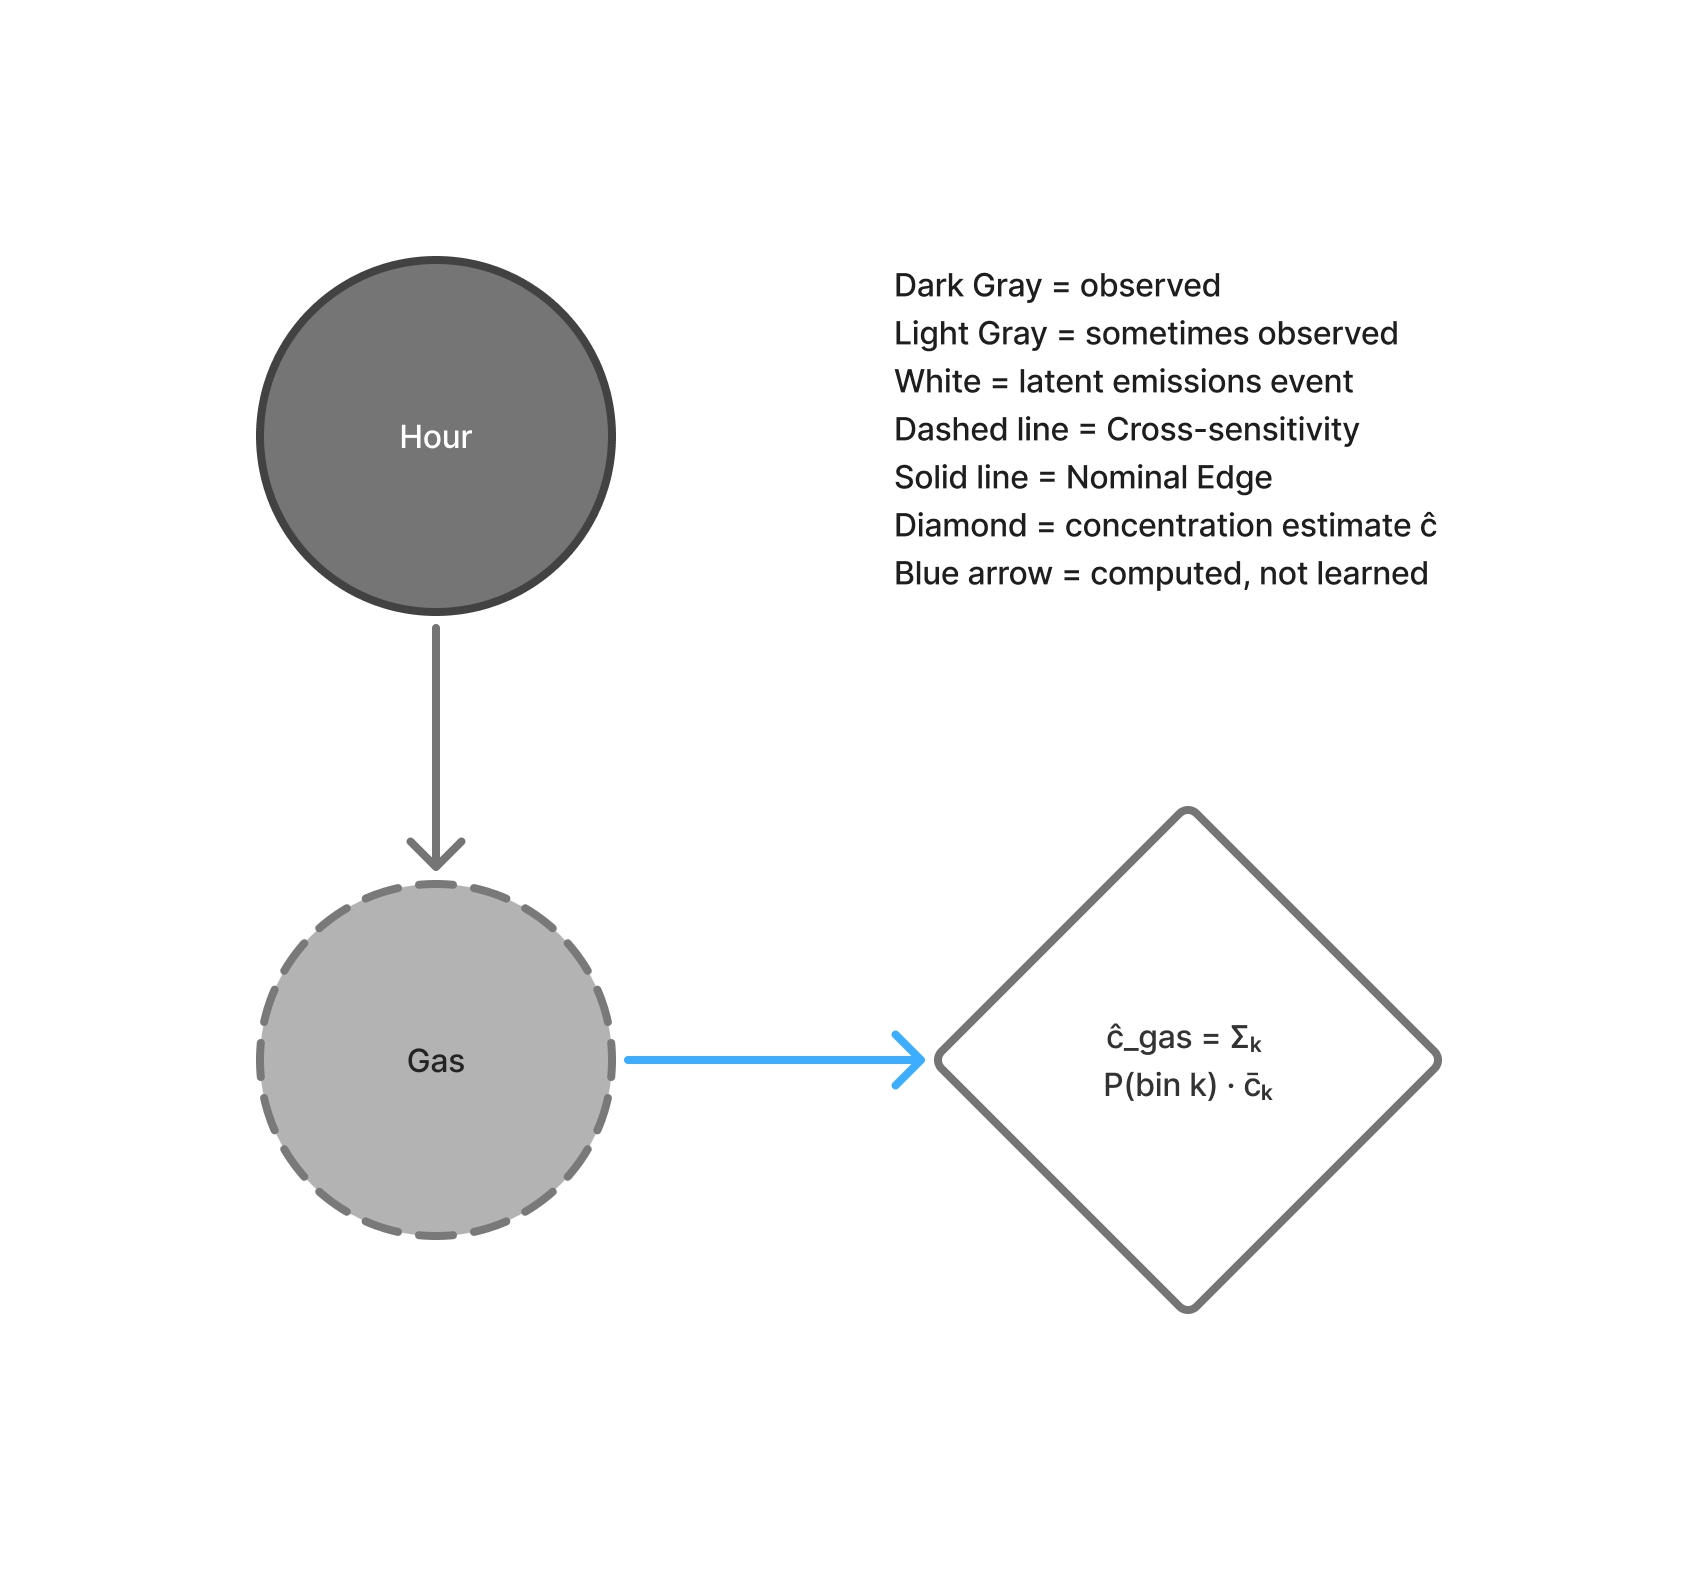
\includegraphics[width=\linewidth,height=0.25\textheight,keepaspectratio]{phase-0}
    \caption{Hour-only baseline.}
    \label{fig:net-baseline}
  \end{subfigure}\hfill
  \begin{subfigure}[t]{0.48\linewidth}
    \centering
    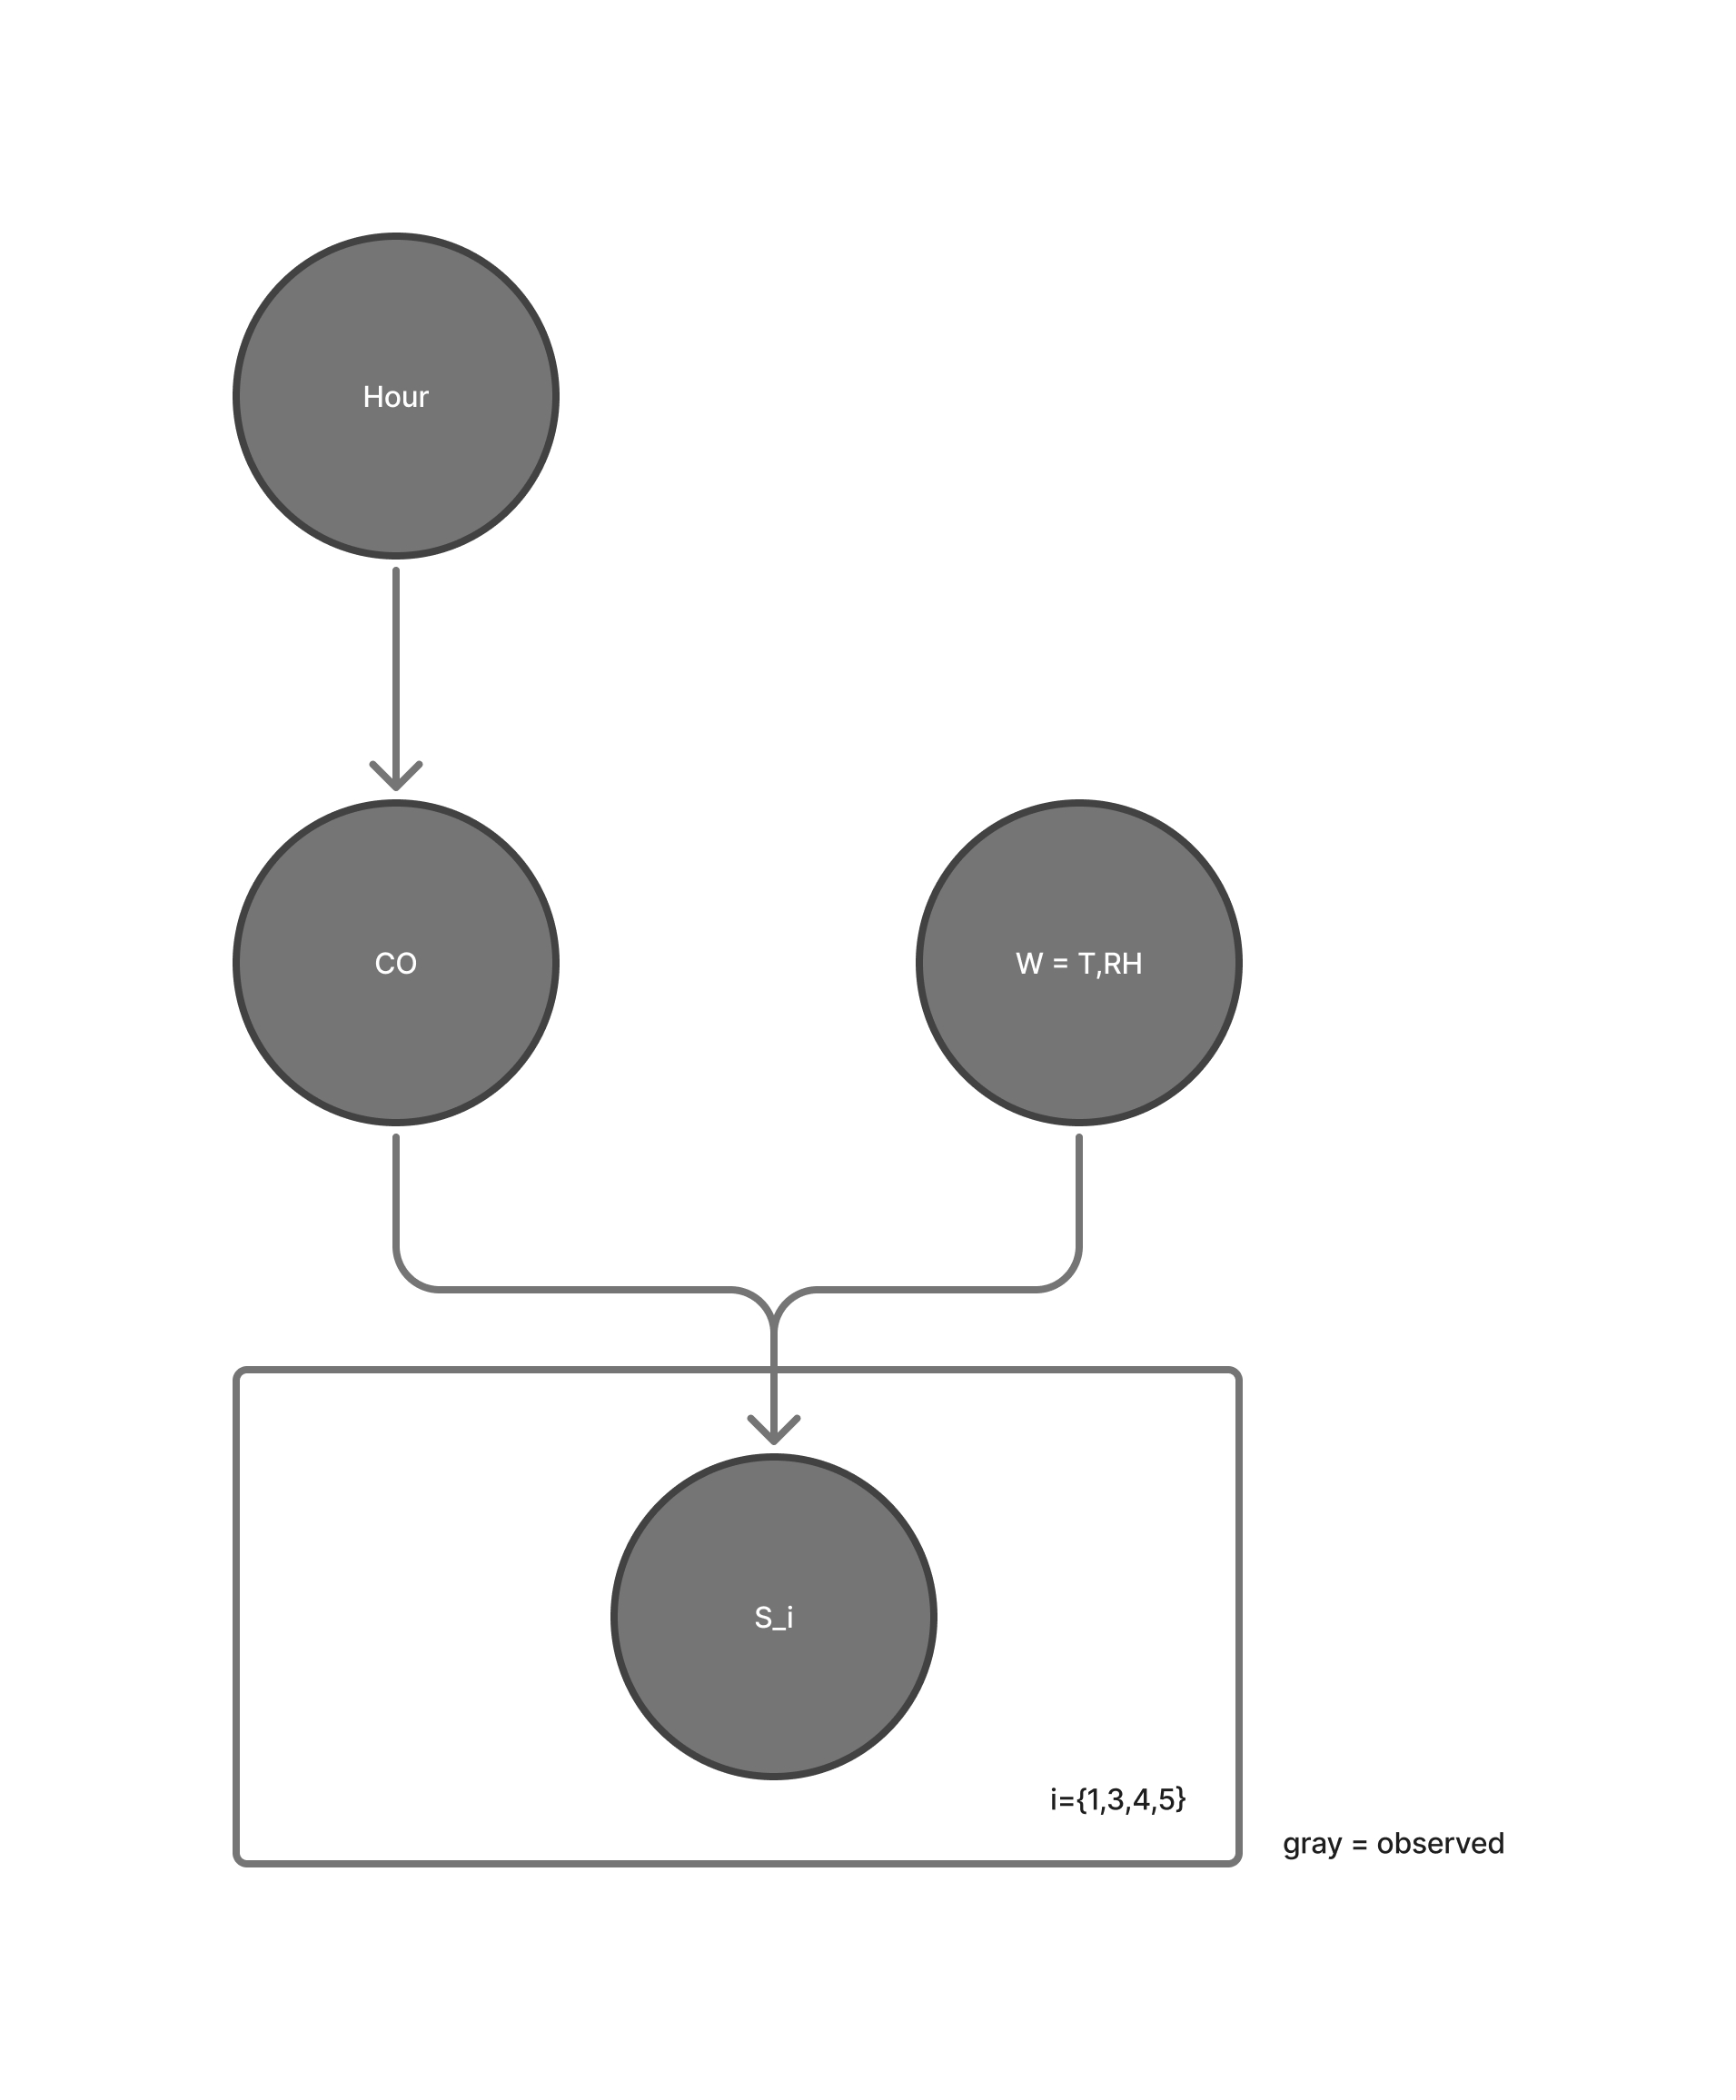
\includegraphics[width=\linewidth,height=0.25\textheight,keepaspectratio]{phase-1}
    \caption{Phase~1: CO only.}
    \label{fig:net-phase1}
  \end{subfigure}

  \vspace{0.8em}
  \begin{subfigure}[t]{0.48\linewidth}
    \centering
    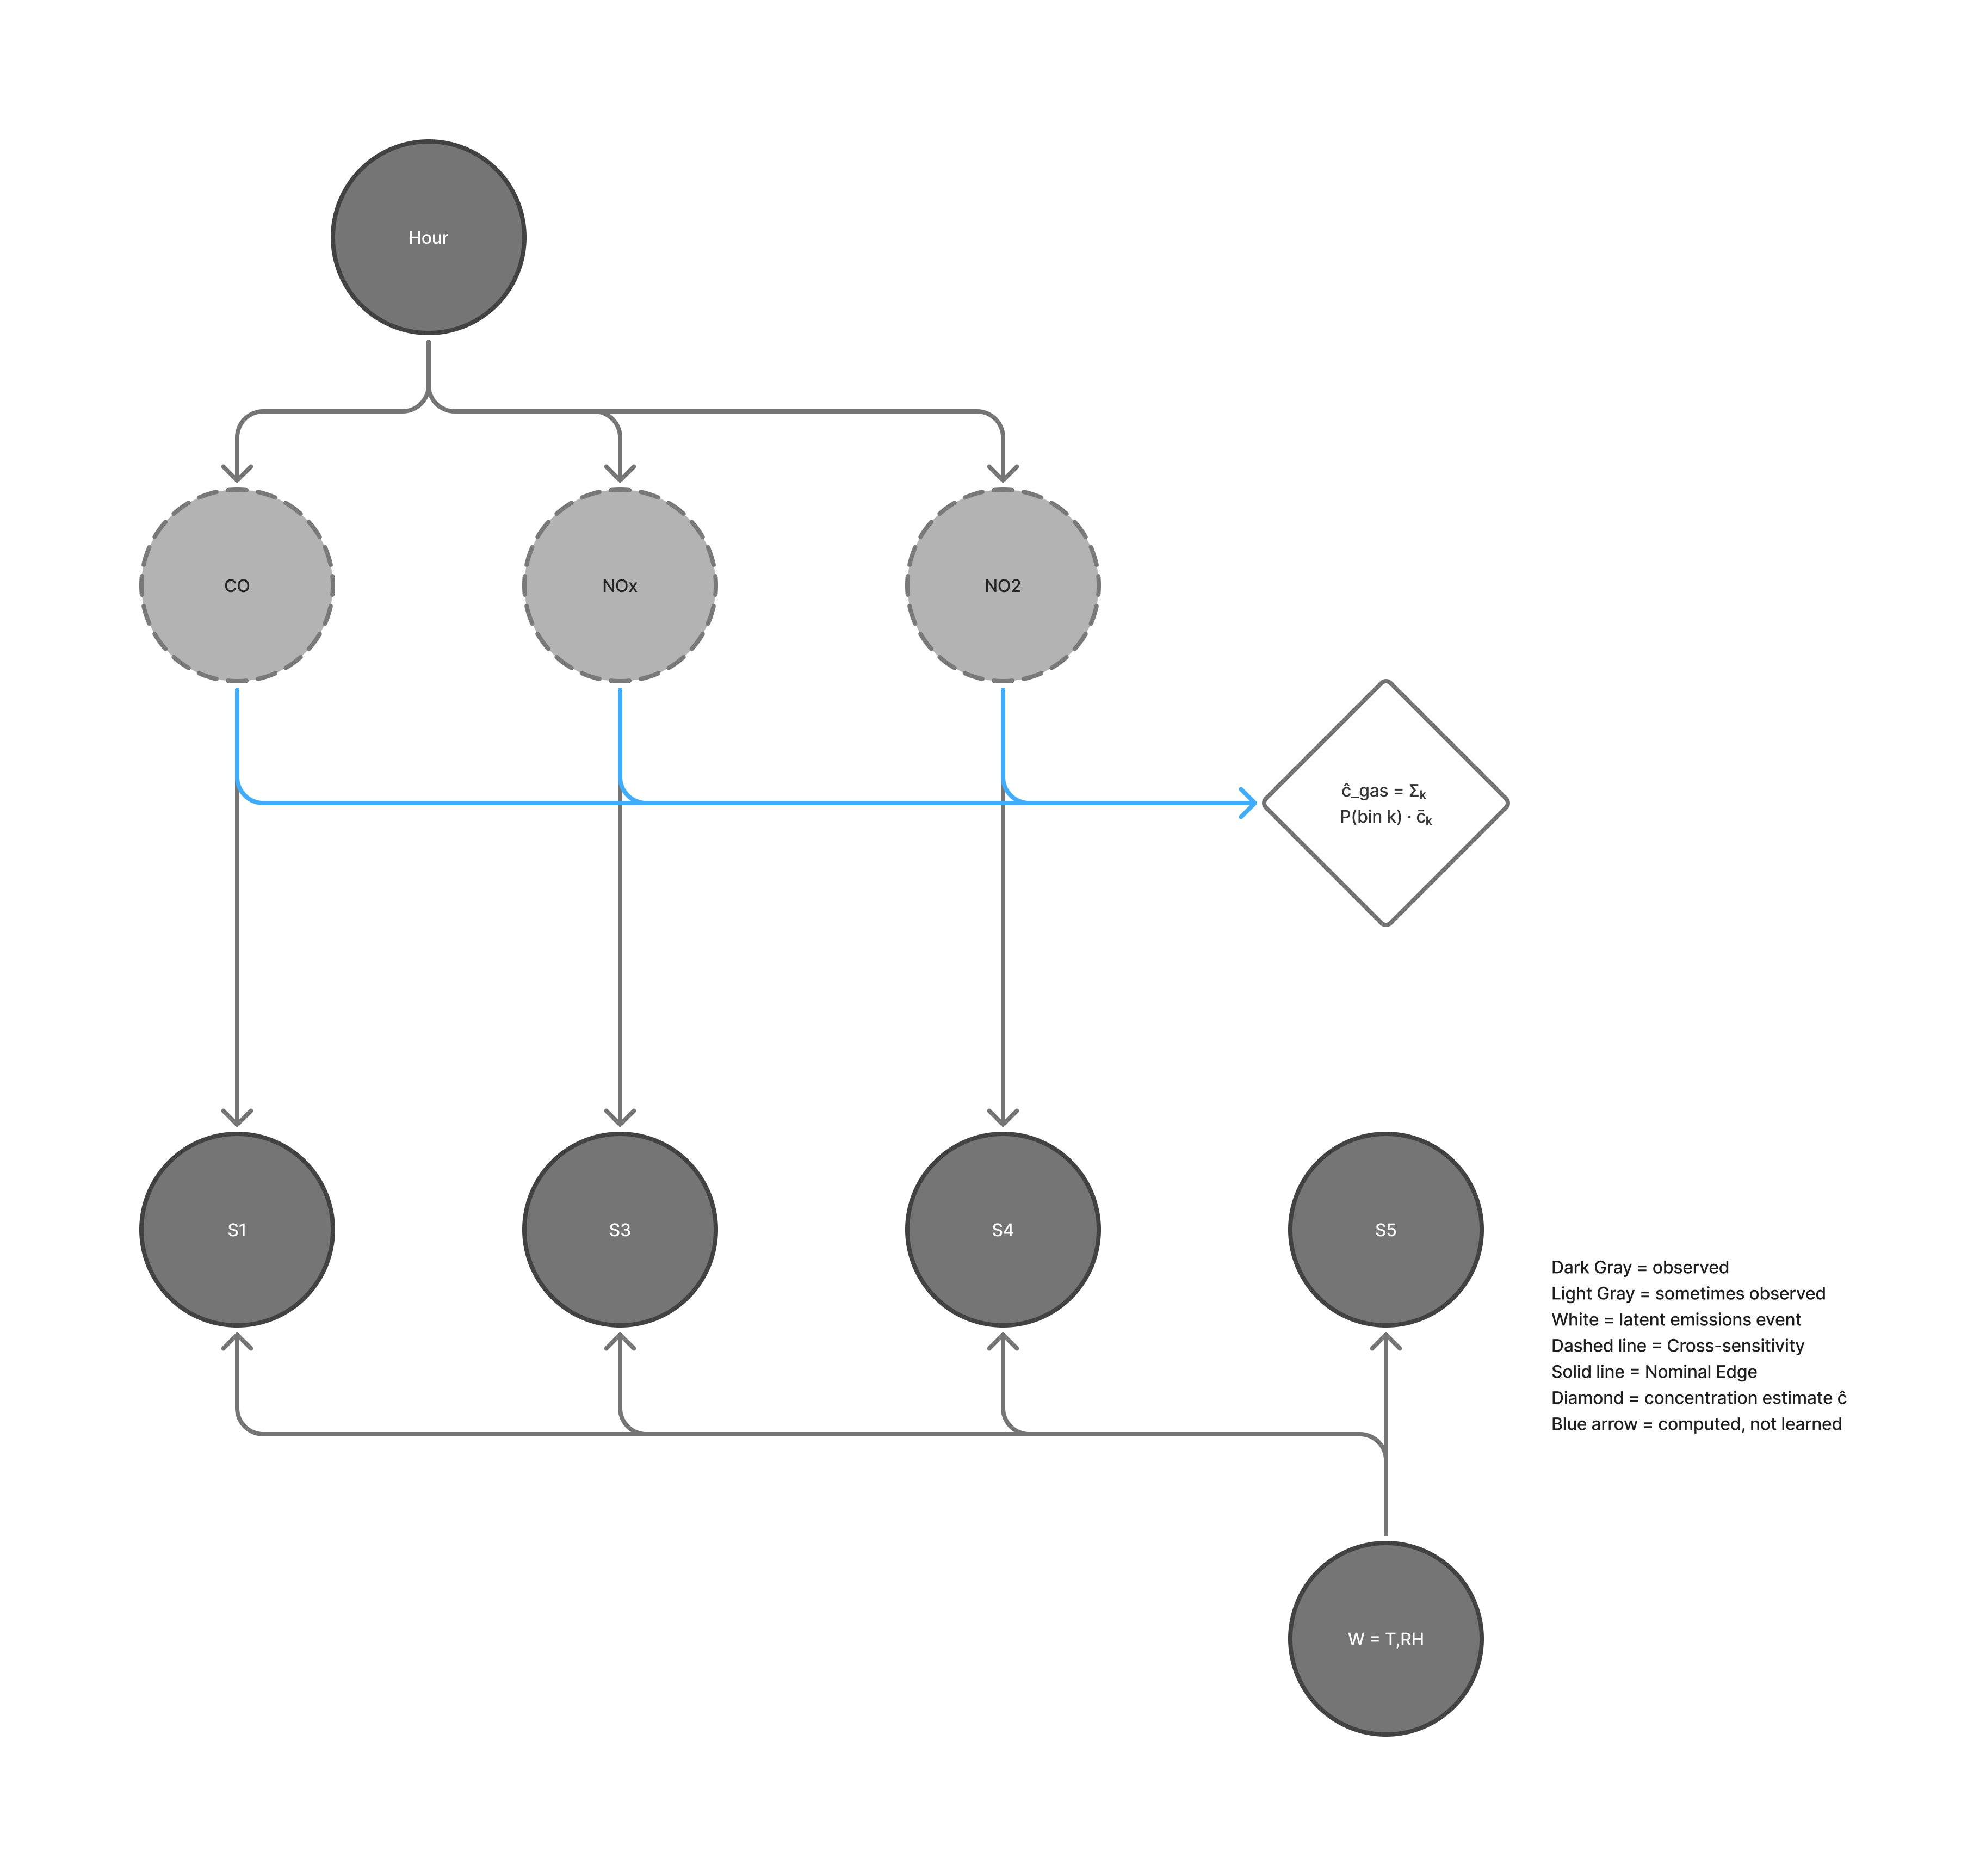
\includegraphics[width=\linewidth,height=0.25\textheight,keepaspectratio]{phase-2}
    \caption{Phase~2: three gases, cross-sensitivities.}
    \label{fig:net-phase2}
  \end{subfigure}\hfill
  \begin{subfigure}[t]{0.48\linewidth}
    \centering
    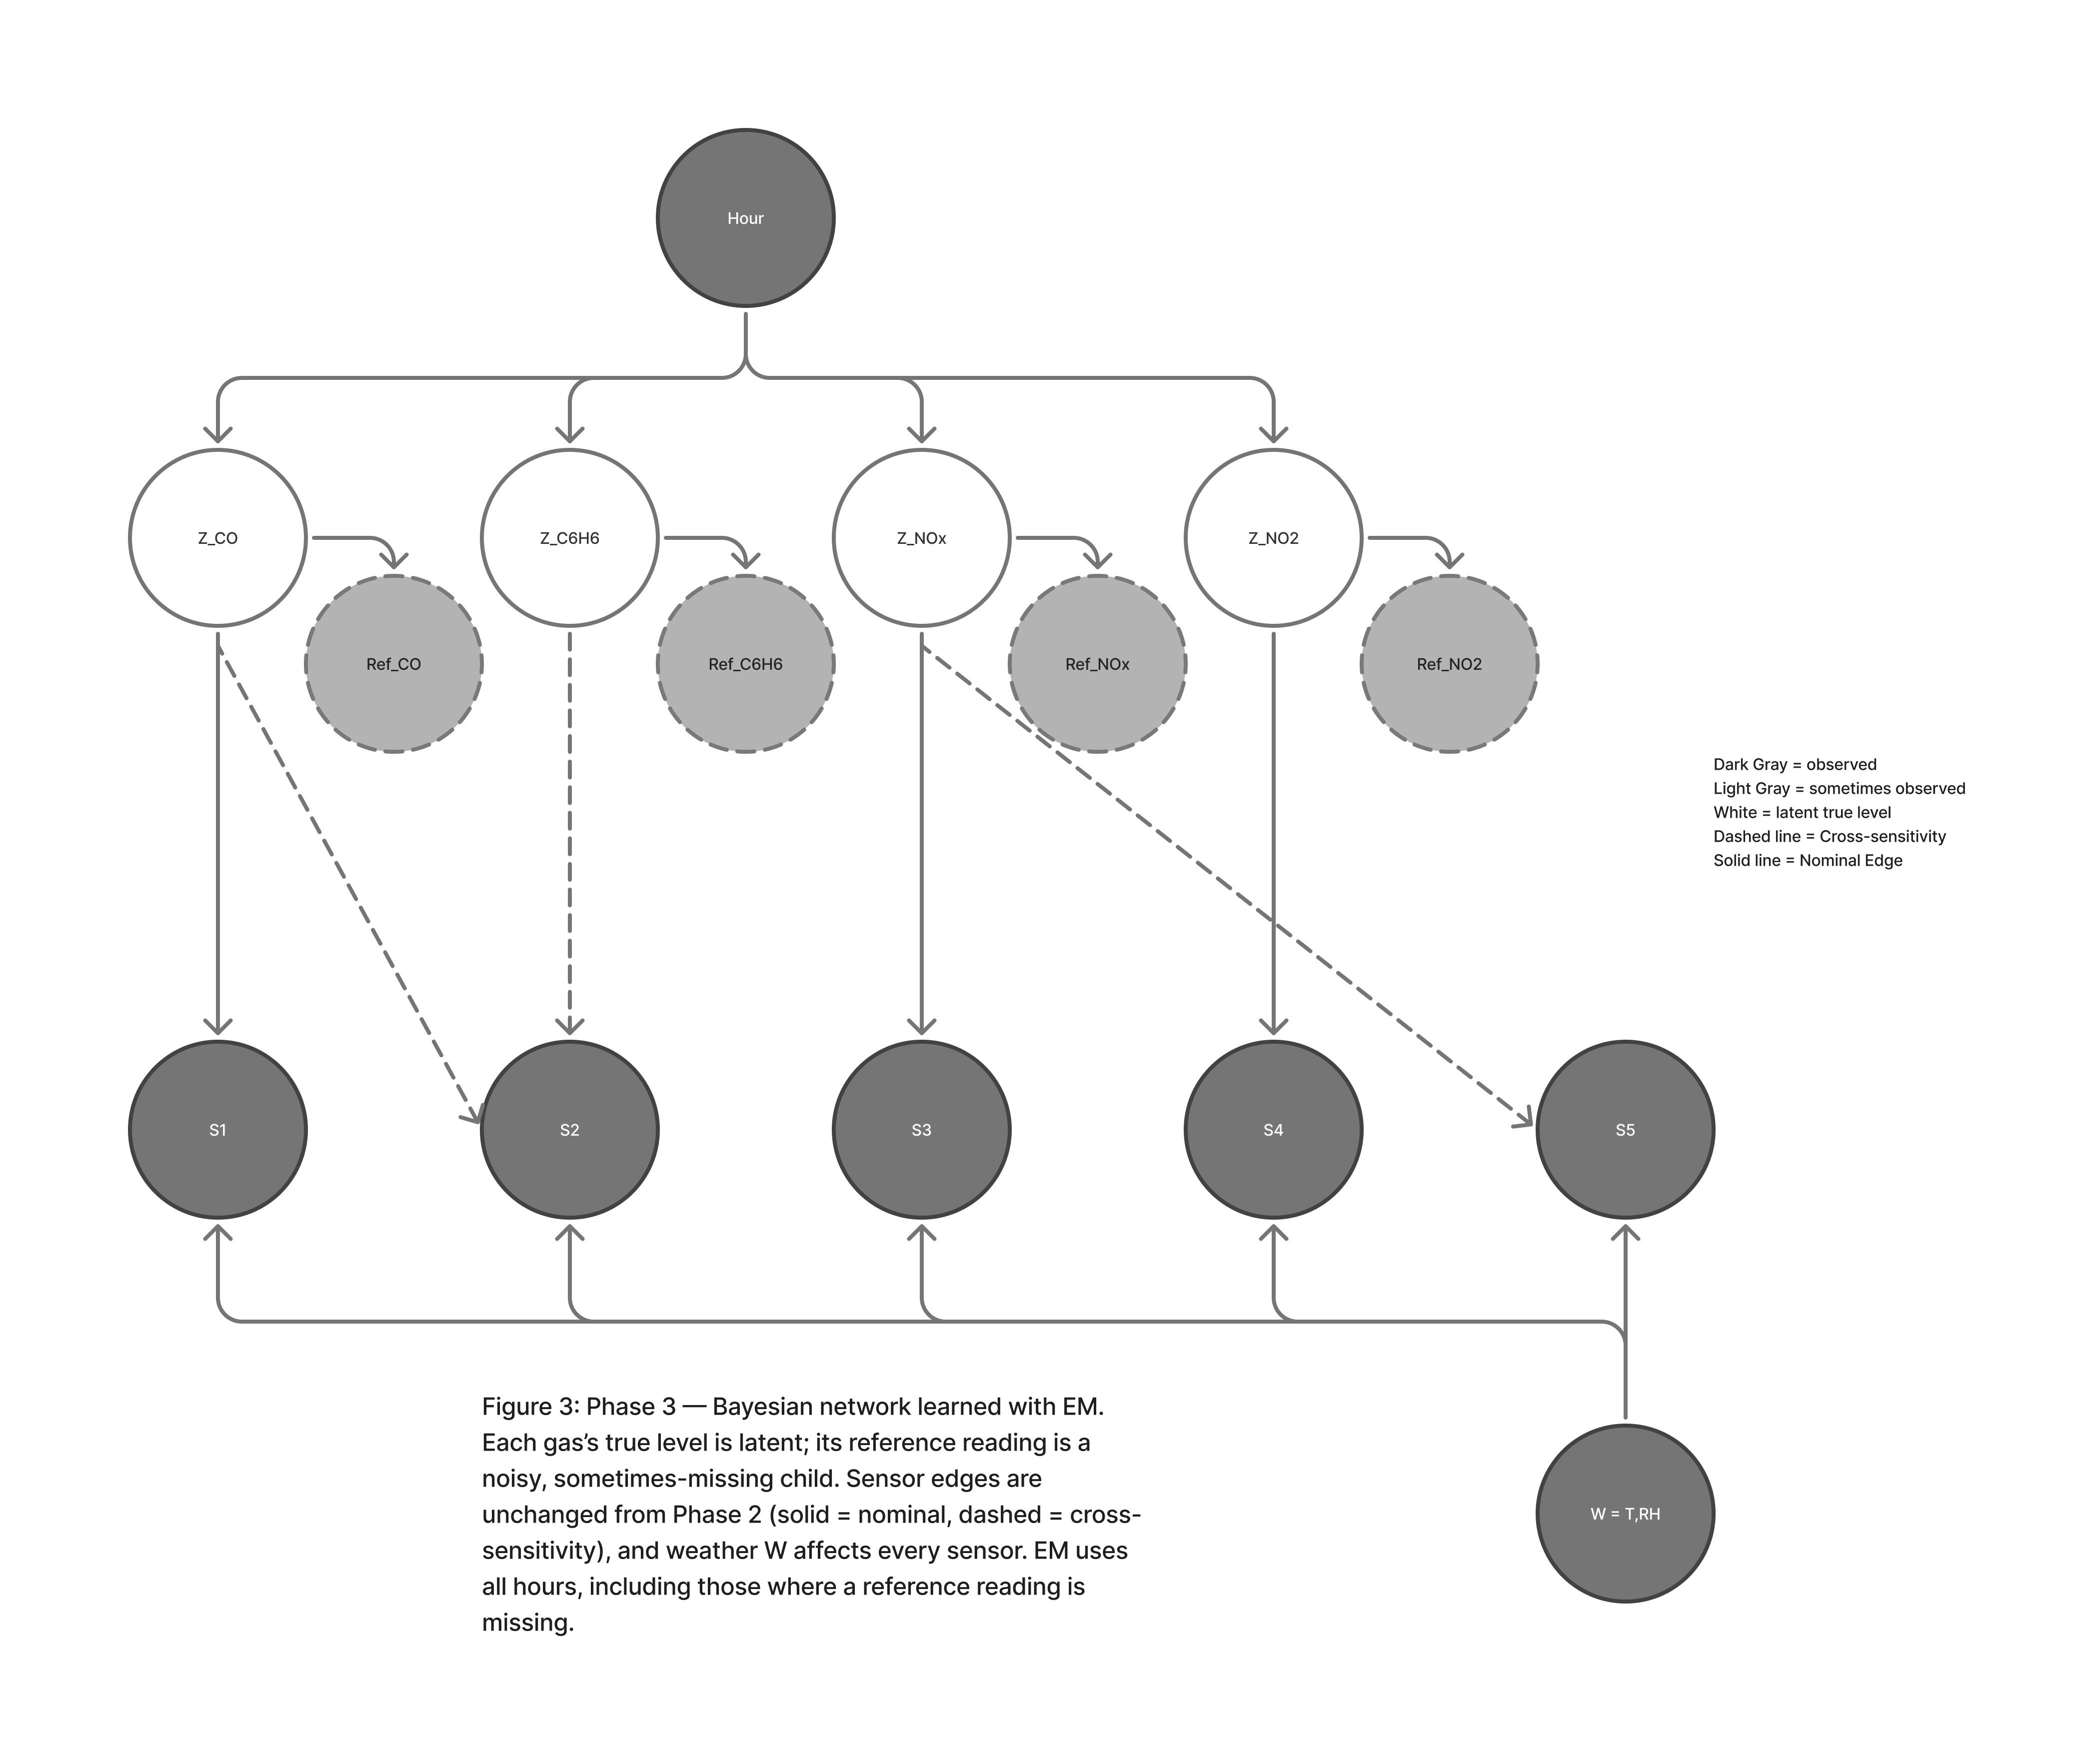
\includegraphics[width=\linewidth,height=0.25\textheight,keepaspectratio]{phase-3a}
    \caption{Phase~3a: \todo{short label}.}
    \label{fig:net-phase3a}
  \end{subfigure}

  \vspace{0.8em}
  \begin{subfigure}[t]{0.48\linewidth}
    \centering
    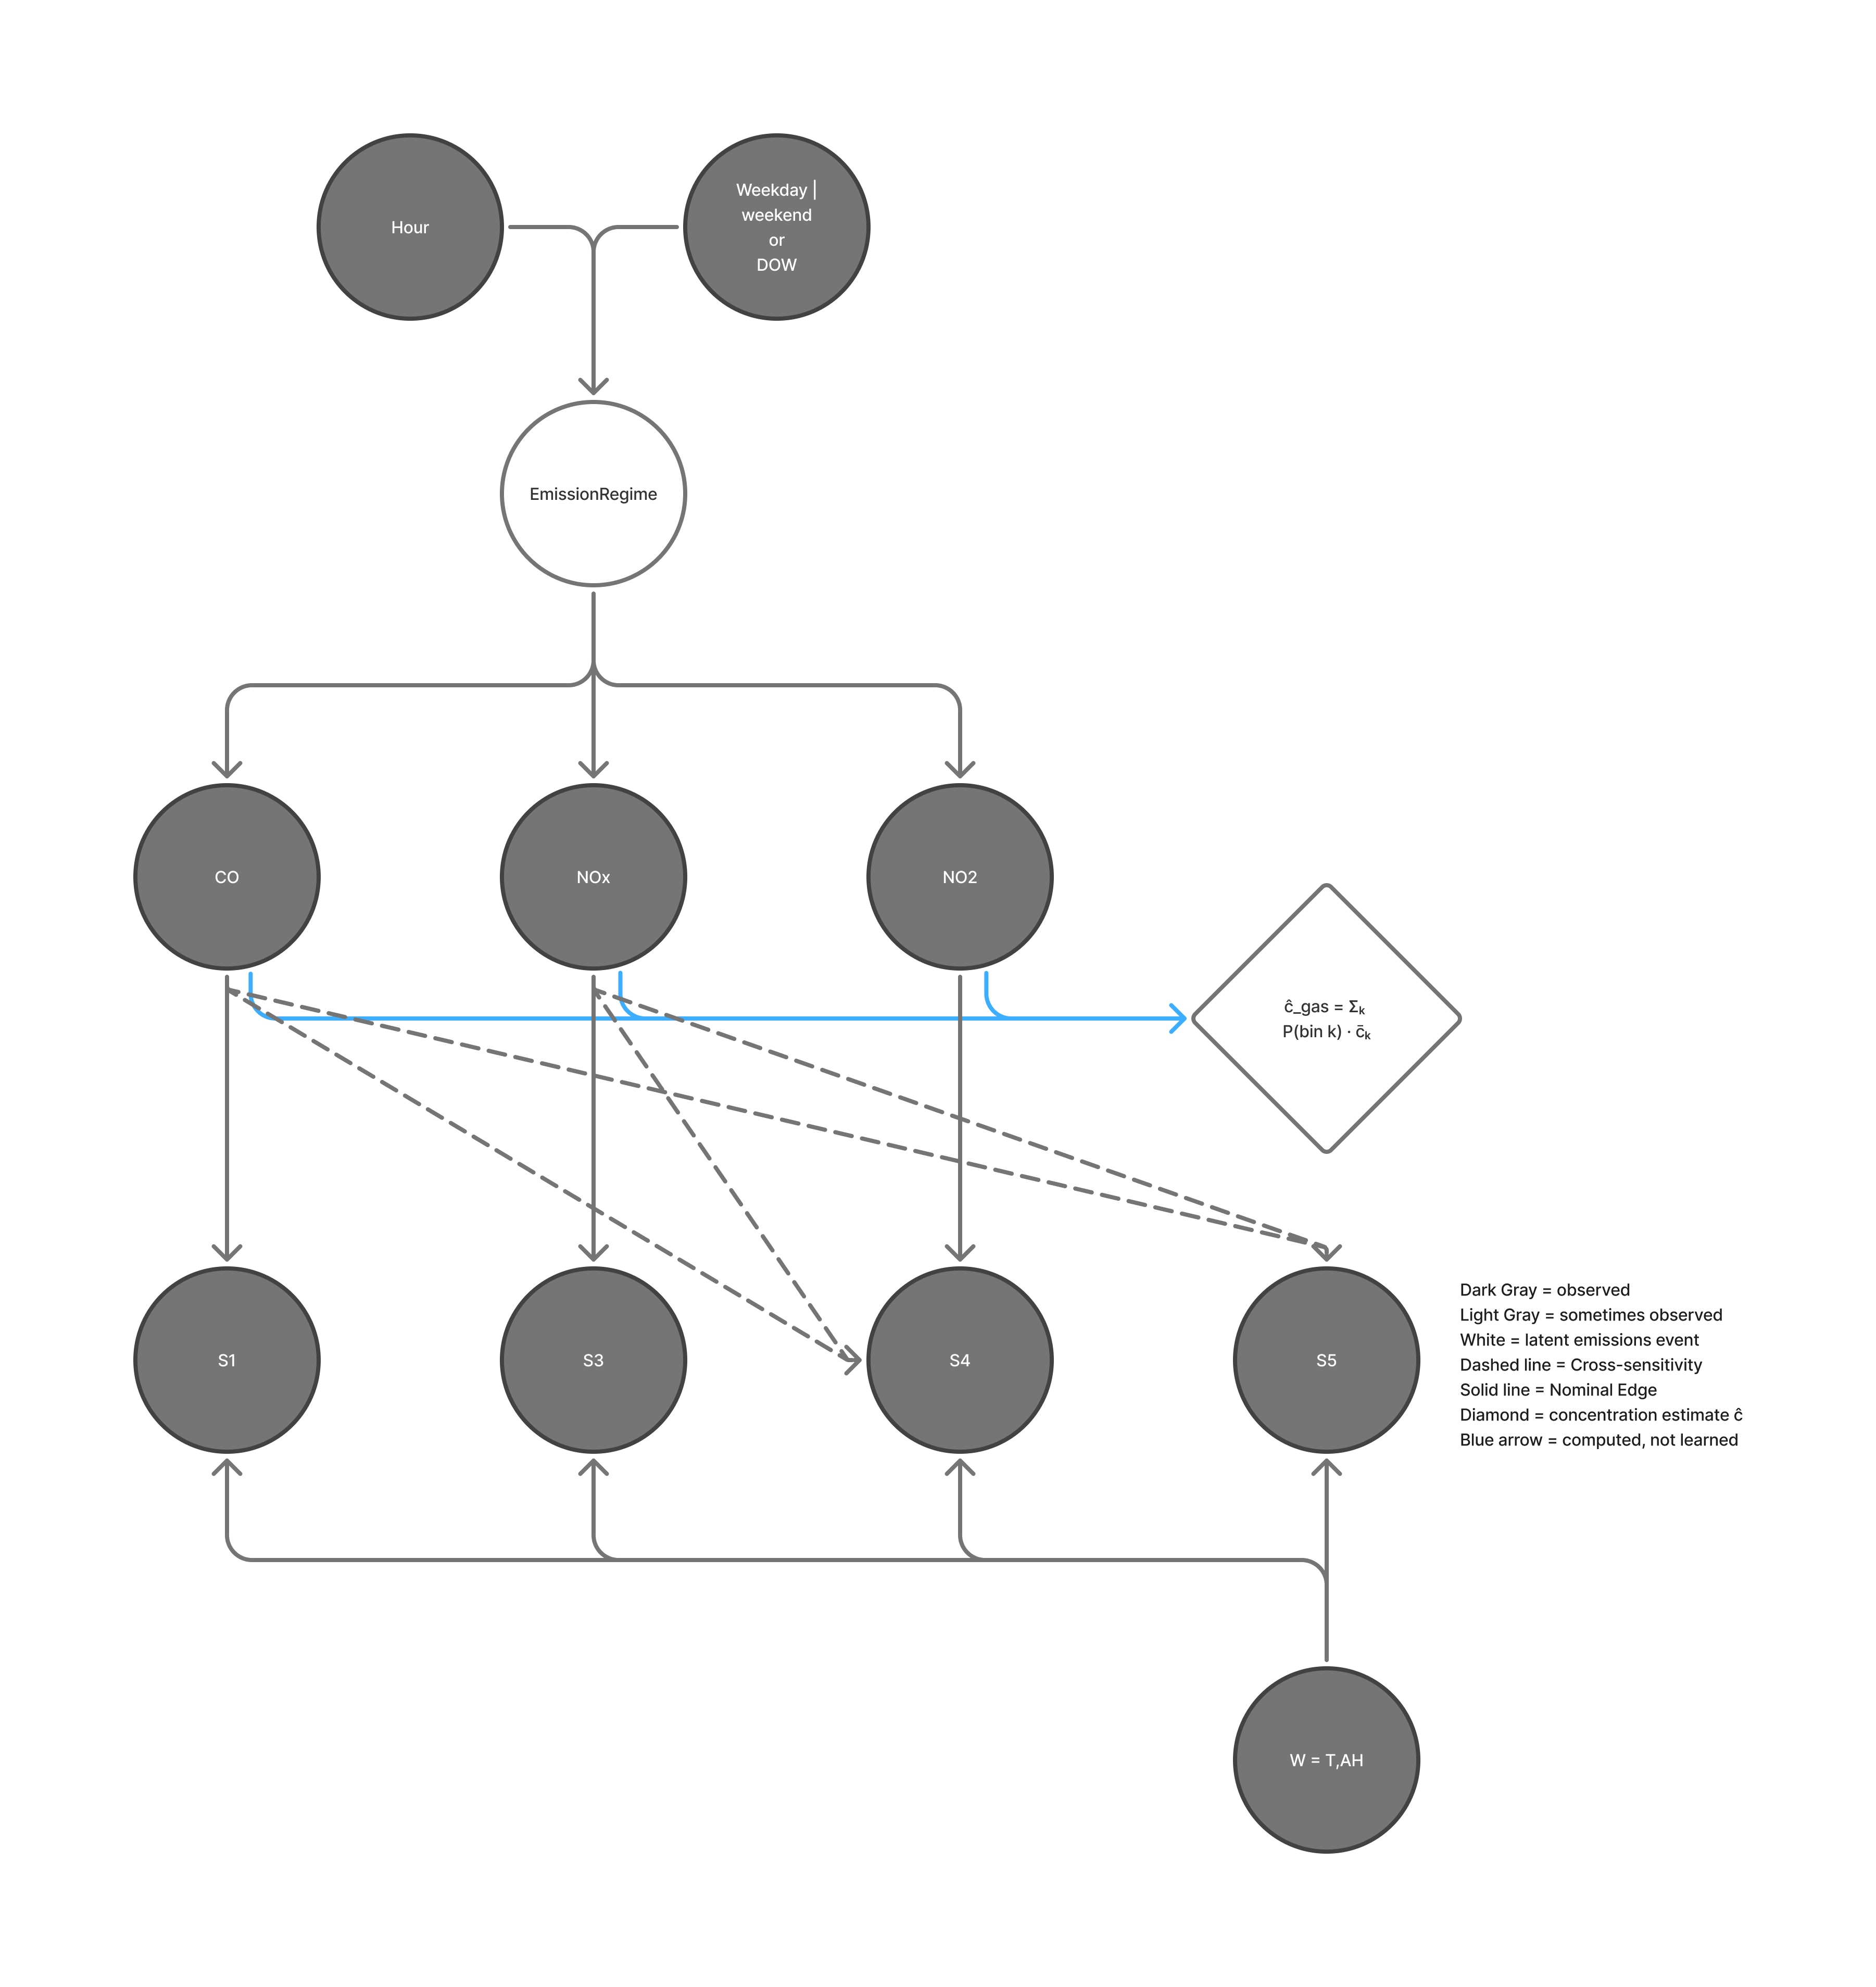
\includegraphics[width=\linewidth,height=0.25\textheight,keepaspectratio]{phase-3b}
    \caption{Phase~3b: latent emission regime (final; also \cref{fig:network}).}
    \label{fig:net-phase3b}
  \end{subfigure}
  \caption{Network for each phase, from the hour-only baseline to the final model.}
  \label{fig:net-variants}
\end{figure}

\section{Missing Data}
\label{app:missing}

\begin{figure}[h]
  \centering
  \begin{subfigure}[t]{0.48\linewidth}
    \centering
    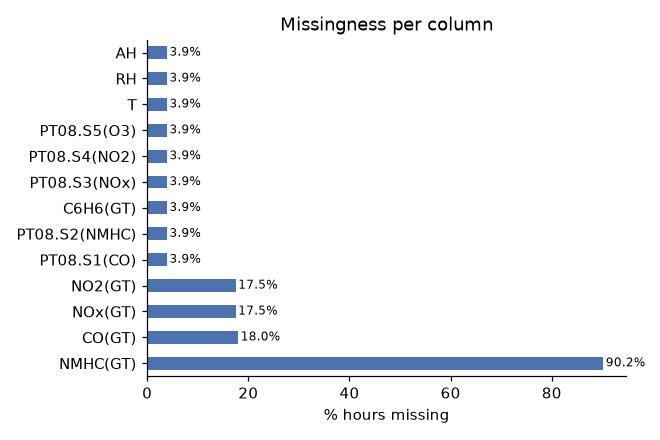
\includegraphics[width=\linewidth]{muska/missingness}
    \caption{Share of hours missing, per column.}
    \label{fig:missing-col}
  \end{subfigure}\hfill
  \begin{subfigure}[t]{0.48\linewidth}
    \centering
    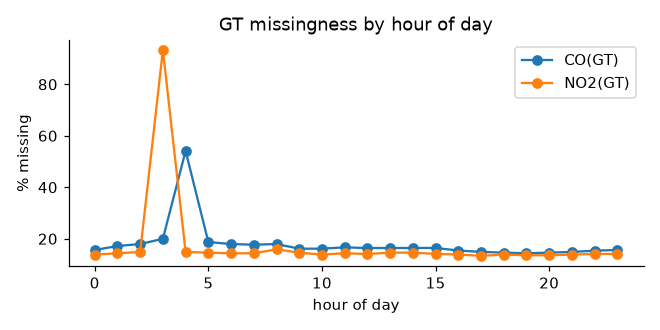
\includegraphics[width=\linewidth]{muska/missing_by_hour}
    \caption{Reference gaps by hour of day.}
    \label{fig:missing-hour}
  \end{subfigure}
  \caption{Missing data. Sensors and weather go missing together (device
  outages); the reference gases are missing far more often, mostly at night.}
  \label{fig:missing}
\end{figure}

\section{Cross-Sensitivity Study}
\label{app:cross}

\paragraph{Why raw correlation is not enough.} CO, NO$_x$ and NO$_2$ all come
from traffic and are strongly correlated with each other (Spearman
$\rho \approx 0.7$--$0.9$), so every sensor looks correlated with every gas.
A gas earned an edge to a sensor only if it explained the sensor beyond the
sensor's nominal gas, the weather and the hour.

\paragraph{Method.} For each sensor we ran forward selection over the candidate
gases on three split seeds. At each step the best candidate was kept only if
(i) adding it as a parent raised the sensor CPT's validation log-likelihood by
at least 0.02 nats per hour on average and in every seed, and (ii) its partial
Spearman correlation with the sensor, controlling for the current parents,
weather and hour, had magnitude at least 0.1 with the same sign in every seed.
We allowed at most two gas parents beyond the nominal one. The study used
$W = (T, \mathit{AH})$; the final network uses $(T, \mathit{RH})$.

\paragraph{Benzene is not an independent reference.} C$_6$H$_6$(GT) is an
almost exact cubic function of $S_2$ ($R^2 \approx 0.99998$) and is missing on
exactly the same hours. Its partial correlation with each other sensor equals
$S_2$'s own and drops to about 0.01 once $S_2$ is controlled for, so it carries
no information beyond $S_2$. We excluded it, and with it $S_2$.

\paragraph{Results.} \Cref{tab:cross} lists the kept edges and the notable
rejections. $S_4$ responds more to CO than to its nominal NO$_2$, which is why
NO$_2$ is the hardest gas to estimate. $S_5$, whose nominal O$_3$ has no
reference, behaves like a general traffic sensor. Several edges with high raw
correlation were rejected (for example $S_1 \leftarrow$ C$_6$H$_6$, raw
$\rho = 0.88$; $S_5 \leftarrow$ NO$_2$, $0.78$), because two sensors with a
common gas parent look correlated even though neither responds to the other's
gas. Some rejected edges keep a nonzero partial correlation but no reliable
likelihood gain at three bins; these are the unmodeled shared signals that can
make the posterior overconfident (\cref{sec:bn}).

\begin{table}[h]
  \centering
  \caption{Cross-sensitivity candidates (mean over three split seeds).
  $\Delta$LL: gain in validation log-likelihood per hour from adding the gas.}
  \label{tab:cross}
  \begin{tabular}{llrrl}
    \toprule
    Sensor & Gas (given) & Partial $\rho$ & $\Delta$LL (nats/h) & Decision \\
    \midrule
    $S_4$ & CO (NO$_2$)             & 0.67  & $0.157 \pm 0.022$ & kept \\
    $S_4$ & NO$_x$ (NO$_2$, CO)     & $-0.50$ & $0.033 \pm 0.002$ & kept \\
    $S_5$ & CO (none)               & 0.85  & $0.403 \pm 0.026$ & kept \\
    $S_5$ & NO$_x$ (CO)             & 0.43  & $0.052 \pm 0.014$ & kept \\
    \midrule
    $S_1$ & NO$_2$ (CO)             & 0.24  & $0.001 \pm 0.024$ & rejected \\
    $S_3$ & CO (NO$_x$)             & $-0.34$ & $0.058 \pm 0.036$ & rejected \\
    $S_3$ & NO$_2$ (NO$_x$)         & $-0.34$ & $0.018 \pm 0.024$ & rejected \\
    $S_5$ & NO$_2$ (CO, NO$_x$)     & 0.27  & $-0.012 \pm 0.003$ & rejected \\
    \bottomrule
  \end{tabular}
\end{table}

\begin{figure}[h]
  \centering
  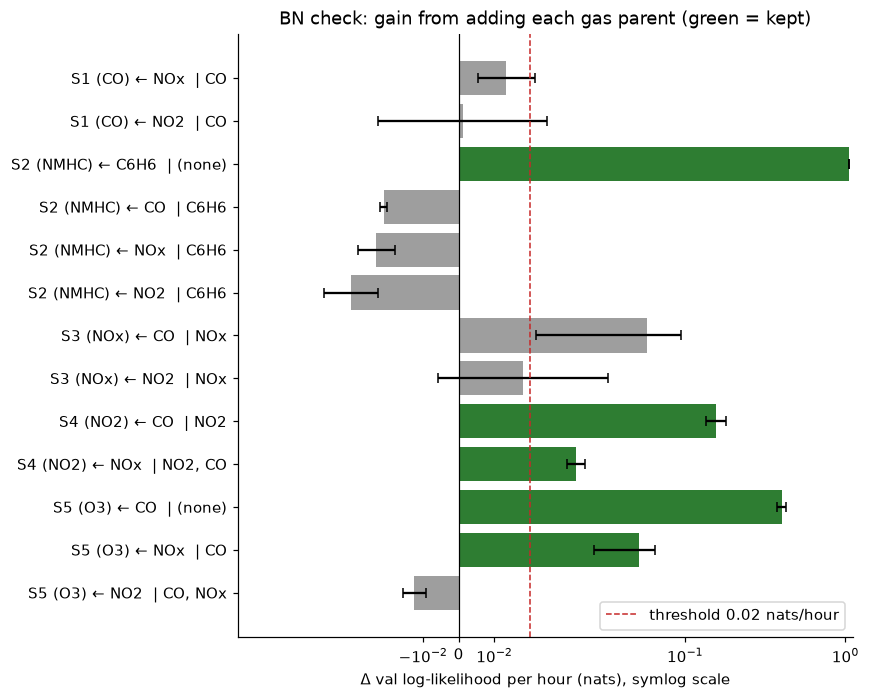
\includegraphics[width=0.7\linewidth]{studies/cross_sensitivity/bn_loglik_gain}
  \caption{Gain in validation log-likelihood from adding each candidate gas
  parent (mean $\pm$ std over three seeds; green = kept; dashed line = 0.02
  nats/h threshold).}
  \label{fig:cross-gain}
\end{figure}

\section{Code and Results}
\label{app:code}
All code and results are at \url{https://github.com/kberesfo/CSE-250A-Project}.
The final runs are the executed notebooks in \texttt{notebooks/<phase>/eval.ipynb}
and \texttt{notebooks/studies/}, which GitHub displays with their outputs;
generated tables and HTML reports are in \texttt{results/}, and figures in
\texttt{figures/}. To reproduce them, open the repository in its dev container,
download the data, and rerun every notebook on a fresh kernel:
\begin{verbatim}
uv run python scripts/get_data
make
\end{verbatim}


\end{document}
